%%% File encoding: UTF-8
%% äöüÄÖÜß  <-- no German Umlauts here? Use an UTF-8 compatible editor!

%%% Magic comments for setting the correct parameters in compatible IDEs
% !TeX encoding = utf8
% !TeX program = pdflatex 
% !TeX spellcheck = de_DE
% !BIB program = biber

\documentclass[master,german]{hgbthesis}
% Permissible options in [..]: 
%   Type of work: diploma, master (default), bachelor, internship 
%   Main language: german, english (default)
%%%----------------------------------------------------------

\RequirePackage[utf8]{inputenc}		% Remove when using lualatex or xelatex entfernen!
\usepackage{graphicx}
\usepackage{svg}
\usepackage{minted}
\usepackage{listings}
\usepackage{varioref}
\usepackage{longtable}
\usepackage{tabularx}
\geometry{top=2.5cm,left=3.5cm,bottom=2.5cm,right=3.5cm}

% -----------------------------------------------------
\newenvironment{code}{\captionsetup{type=listing}}{}
% -----------------------------------------------------
% -----------------------------------------------------
\newcommand{\mysubsubsection}[1]{{\subsubsection{\textbf{#1}}}}
\newcommand{\mentionedtext}[1]{{\textit{{#1}}}}
\newcommand{\sourceDir}{./sources}
\newcommand{\sourceFontSize}{\fontsize{10pt}{11.5}}
\newcommand{\quotes}[1]{``#1''}
\newmintedfile[bashFile]{bash}{
	linenos=false, 
	frame=none, 
	breaklines=true, 
	tabsize=2,
	numbersep=5pt,
	xleftmargin=10pt,
	baselinestretch=1,
	fontsize=\sourceFontSize
}
\newmintedfile[yamlFile]{yaml}{
	linenos=false, 
	frame=none, 
	breaklines=true, 
	tabsize=2,
	numbersep=5pt,
	xleftmargin=10pt,
	baselinestretch=1,
	fontsize=\sourceFontSize
}
\newmintedfile[javaFile]{java}{
	linenos=false, 
	frame=none, 
	breaklines=true, 
	tabsize=2,
	numbersep=5pt,
	xleftmargin=10pt,
	baselinestretch=1,
	fontsize=\sourceFontSize
}
\newmintedfile[xmlFile]{xml}{
	breaklines=true, 
	tabsize=2,
	numbersep=5pt,
	xleftmargin=10pt,
	baselinestretch=1,
	autogobble=true,
	breakautoindent=false,
	fontsize=\sourceFontSize
}
\newmintinline[inlineJava]{java}{
	fontsize=\sourceFontSize
}
\newmintinline[inlineBash]{bash}{
	fontsize=\sourceFontSize
}
% -----------------------------------------------------
\graphicspath{{images/}}    % location of images and graphics
\logofile{logo}				% logo file = images/logo.pdf (use \logofile{} for no logo)
\bibliography{references.bib}  	% name of bibliography file (references.bib)
\setlength{\parindent}{0pt}

%%%----------------------------------------------------------
% Title page entries
%%%----------------------------------------------------------

%%% Entries for ALL types of work: --------------------------
\title{Implementierung einer Partnerdatenbank und Evaluierung des verwendeten Technologiestack} %no camel used (and Camel)
%\author{Ing. Thomas Herzog B.Sc}
%\programname{Software Engineering}
\placeofstudy{Hagenberg}
\dateofsubmission{2020}{05}{30}	% {YYYY}{MM}{DD}

%%% Entries for Bachelor theses only: -----------------------
%\thesisnumber{XXXXXXXXXX-A}   %e.g. 1310238045-A  
% (Stud-ID, A = 1st Bachelor thesis)
%\semester{Fall Semester 2017} 	% Fall/Spring Semester YYYY
%\coursetitle{Introduction to Trivial Problems 1} 
\advisor{FH-Prof. DI Dr. Herwig Mayr}

%%% Restricted publication license instead of CC (master only):
%\cclicense

%%%----------------------------------------------------------
\begin{document}
%%%----------------------------------------------------------

%%%----------------------------------------------------------
\frontmatter							% title part (roman page numbers)
%%%----------------------------------------------------------

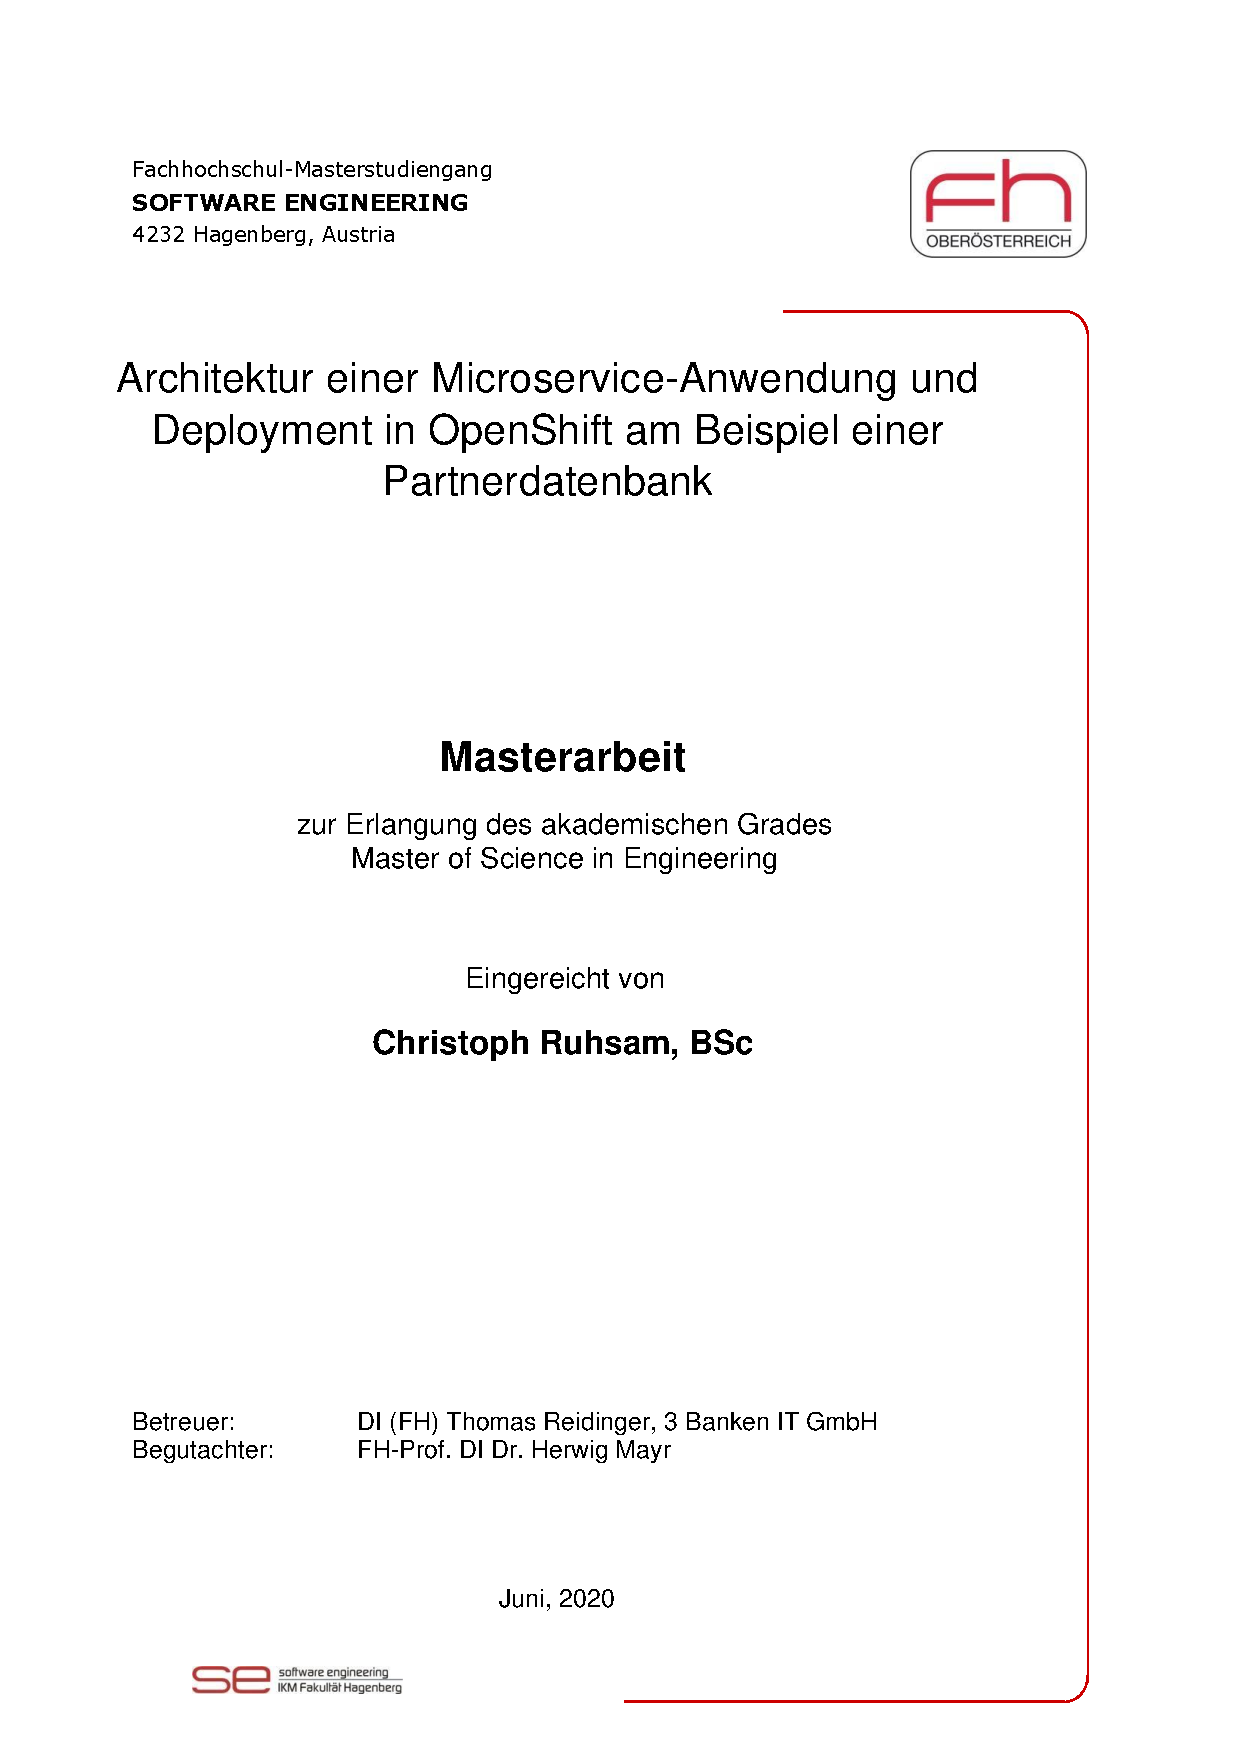
\includepdf{title.pdf}
%\maketitle
\tableofcontents

%\chapter{Preface}






 	% preface is optional
\chapter{Abstract}
An Enterprise Service Bus (ESB) is a crucial part of an enterprise, which connects the enterprise to its partners, customers, and other branches. The appearance of containerization, cloud services, and the microservice architecture have provided new possibilities for implementing and running an ESB. But, an ESB is commonly used by large conservative enterprises, which don't adapt new technologies fast, and wait until a new technology has proven itself. Especially the cloud is something the industry denied to use for a long time, because of the fact, that the infrastructure and data are managed and maintained by external service providers. \\ 

These days, we live in the so called cloud age, whereby global enterprises like Red Hat or Amazon provide cloud services such as Platform as a Service (PaaS), which can scale with the business. Enterprises start to consider to move their ESB installations to the cloud to profit from the cloud service provided features. Moving an ESB to the cloud will be a long term process for an enterprise, because the established processes for development, running, and managing the ESB will have to change. \\

This thesis has the goal to give the reader an overview of the cloud related concepts and technologies such as, Infrastructure as Code (IaC) and Docker, which are the base for cloud services. The implemented ESB prototype,  is  available at \url{https://github.com/cchet-thesis-msc/prototype}, and shows how an ESB could be implemented on a PaaS platform. \\




%%%----------------------------------------------------------
\mainmatter          			% main part (arabic page numbers)
%%%----------------------------------------------------------

\chapter{Introduction}
\label{cha:intro}

\section{Motivation}
\label{sec:intro-motivation}
Large enterprises work with several independent applications, whereby each application covers an aspect of their business. In general, these applications are from different vendors, implemented in different programming languages, and with their own life-cycle management. To provide a business value to the enterprise, these applications are connected via a network and they contribute to a business workflow. The applications have to exchange data, which is commonly represented in different formats and versions. This leads to a highly heterogeneous network of applications, which is hard to maintain. \\

The major challenge of an IT department is the integration of independent applications into the enterprise application environment. The concept of Enterprise Application Integration (EAI) provides patterns, which help to define a process for the integration of applications into a heterogeneous enterprise application environment. One of these patterns is the Enterprise Service Bus (ESB), which is widely used in the industry\cite{EIP}. \\

Often, the term ESB application is used to refer to an ESB, which integrates internal and external hosted applications. But an ESB is a software architectural model rather than an application. The term could have been established by the usage of middleware such as JBoss Fuse, which provides tooling to integrate applications into an ESB. Red Hat JBoss Fuse is based on the JBoss Enterprise-Application-Platform (JBoss EAP), where all integration services run in the same runtime environment\cite{Fuse2018}. \\

With the appearance of cloud services such as Platform as a Service (PaaS), it is now possible to move an ESB from a dedicated environment to a cloud environment, whereby each integration service runs in its own runtime environment, rather than joining an existing runtime environment. The concept of Integration Platform as a Service (IPaaS) is built on top of PaaS, and enhances a common PaaS service with the integration features required by EAI\cite{PaaS2015, iPaaSP12015}. \\

Thus, enterprises can reduce the effort in implementing and maintaining an ESB, integrating applications via the ESB, and reducing the costs of an ESB, by using a consumption based pricing model. The cost are reduced due to the fact, that the ESB can scale down when its load decreases, whereby less resources are consumed, which have to be paid for.

\section{Objectives}
\label{sec:intro-objectives}
This thesis aims to implement an ESB on Openshift PaaS. An ESB is different to a Service Hub, because the ESB is a distributed system by design, whereby for instance transformation is not centralized, as it is with a Service Hub. A Service Hub has a central component, which performs transformation, routing and orchestration, whereby the scaling is limited by the hardware capabilities of the central hub. Additionally, the hub component of a Service Hub represents a single point of failure\cite{EIP}. \\

Commonly, an ESB is implemented with the help of middleware such as JBoss Fuse, which is based on JBoss EAP. The concepts of PaaS and IPaaS are in general new to the industry, which commonly hosts their integration services in their own data centers, due to the lack of trust for cloud services and knowledge about the new approaches such as the microservice architecture\cite{Openshift2018}. \\

Before implementing an ESB, which runs on a PaaS platform such as Openshift, it is necessary to understand the new concepts such as Infrastructure as Code (IaC) or containerization with Docker, which are covered in the following chapters. The microservice architecture and cloud services such as PaaS are becoming more important for the software industry, because of the features they provide. For instance, Red Hat is currently moving its ESB middleware JBoss Fuse to the cloud, whereby JBoss Fuse will fully rely on Openshift, and the integration services will have to be implemented as microservices. This has a huge impact on Red Hats customers, who are used to JBoss Fuse on top of JBoss EAP. \\

This thesis was commissioned by the company Gepardec IT Services GmbH, a company, which is working in the area of Java Enterprise and Cloud Development. The migration from a monolithic ESB to a microservice structured ESB, which is hosted in a PaaS environment is a major concern for them. The migration from a monolithic ESB to a microservice structured ESB will be a major challenge for their customers, because the microservice architecture and cloud services are mostly new to them.  \\

Over the past years a huge technology dept has been produced by the industry, due to the monolithic architecture of their applications and little refactoring work on their application sources. It will be hard for them to reduce the accumulated technology dept, which they will have to, to keep competitive. Gepardec sees a lot of potential for their business and their customers in this new approach of implementing and hosting an ESB. \\

The term \mentionedtext{monolithic ESB} refers to an ESB implementation, whereby all integration services are part of a single application, and therefore, are part of the application life-cycle, instead of having an own life-cycle per integration service. An integration service is a service, which integrates two or more other service with each other, by handling aspects like data transformation or security between the integrated service and its consumers.  
%\chapter{Infrastructure as Code}
\label{cha:iac}
Infrastructure as Code (IaC) is a concept to automate system creation and change management with techniques from software development. Systems are defined in a Domain Specific Language (DSL), which gets interpreted by a tool, which creates an instance of the system or applies changes to it. IaC defines predefined, repeatable routines for managing systems. IaC descriptors are called templates, cookbooks, recipes, or playbooks, depending on the IaC tool. In the further course, the IaC descriptors will be called templates. The DSL allows to define resources of a system such as network, storage, and routing descriptively in a template. The DSL abstracts the developer from system specific settings and provides a way to define the system with as little configuration as possible\cite{Morris2016}. \\

The term \mentionedtext{system} is used as a general description, whereby in the context of IaC, a system can be anything, which can be described via a DSL. The term \mentionedtext{environment} is also used as a general description for a habitat for one or more systems.  

\section{The Need for Infrastructure as Code}
\label{sec:iac-need}
In the so called iron age, the IT systems were bound to the physical hardware, and the setup of such a system and its change management were a long term, complex, and error prone process. These days, we call such systems legacy systems. In the cloud age, the IT systems are decoupled from the physical hardware, and in the case of PaaS, they are even decoupled from the operating system. The IT systems are decoupled due to the fact, that cloud providers cannot allow their customer to tamper with the underlying hardware and operating system. In general, the hardware resources, provided by a cloud provider, are shared by multiple customers\cite{Morris2016}. \\

With IaC it is possible to work with so called Dynamic Infrastructure Platforms (DIPs), which provide computing resources for a system, whereby the developers are completely abstracted from the underlying infrastructure. DIPs have the characteristic to be programmable, are available on demand, and provide self service mechanisms, therefore, we need IaC to work with such infrastructures. Systems deployed on DIPs are flexible, consistent, automated, and reproducible\cite{Morris2016}. \\

The term \mentionedtext{infrastructure} is used as a general description for the foundation of systems, which provides any kind of resources the systems can consume. \\

Enterprises, which stuck to legacy systems, face the problem that technology nimble competitors can work with their infrastructures more efficiently, and therefore can demand lower prices from their customers. This is due to the IaC principles, which are discussed in Section \vref{sec:iac-principles}. Over a short period of time, enterprises will have to move to IaC and away from their legacy systems to stay competitive. The transition process could be challenging for an enterprise, because they lose control over the physical hardware, and maybe also over the operating system. Maintaining legacy systems has the effect, that someone is close to the system, and almost everything is done manually. IaC has the goal to automate almost everything, which requires trust for the cloud providers, which provide the infrastructure and the tooling. A well known problem, which enterprises will face, is the so called Automation Fear-Spiral, which is shown in Figure \vref{fig:automation-fear-spiral}.

\begin{figure}[htbp]
	\centering
	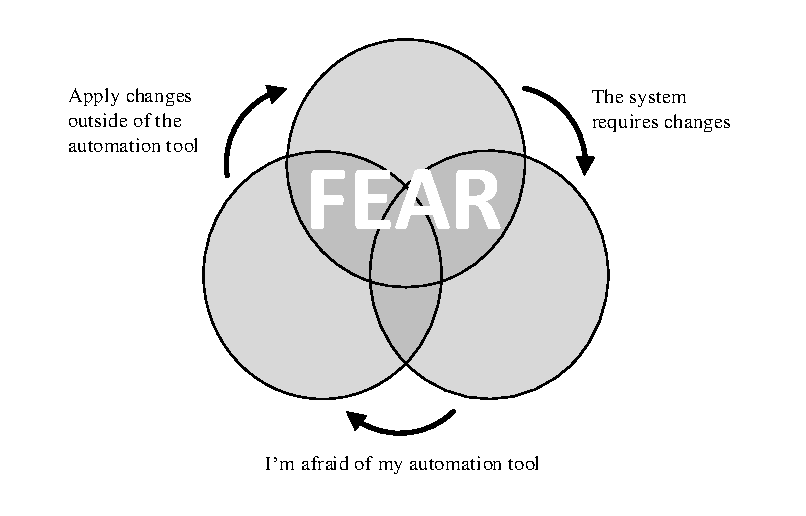
\includegraphics[scale=1]{images/automation-fear-spiral.pdf}
	\caption{Automation Fear-Spiral}
	\label{fig:automation-fear-spiral}
\end{figure} 

Because of no trust for the automation, changes are applied manually to the systems, and outside the defined automation process. If the system is reproduced, definitions maybe missing in the templates, which leads to an inconsistent system. Therefore, enterprises have to break this spiral to fully profit from IaC \cite{Morris2016}. \\

When enterprises have moved their legacy systems to IaC, they can not only manage their systems faster, they also can profit from the principles of IaC as discussed in Section \vref{sec:iac-principles}. With IaC, systems are less complicated to manage, changes can be applied without fear, and the systems can easily be moved between environments. This provides the enterprises with more space to maneuver, whereby the systems can become more complex, but still easy to manage, and the systems can be defined and created faster, which could lower costs.    

\section{Principles of Infrastructure as Code}
\label{sec:iac-principles}
The principles of IaC solve the problems of systems of the iron age. In the iron age the creation and maintenance of systems were a long term, complicated, and error prone process, which consumed a lot of resources and time. With the decoupling of the physical hardware from the systems, the creation and maintenance of systems has become simple, due to the abstraction layer provided by the IaC DSL and tooling. 

\subsection{Systems are Reproducible}
\label{sec:iac-principles-reproducibility}
With IaC, systems are reproducible. It is possible to reproduce a whole system or parts of it effortlessly. Effortless means, that no tweaks have to be made to the templates or during the reproduction process, and there is no need for a long term decision process about what has to be reproduced and how to reproduce it. To be able to reproduce systems effortlessly is a powerful capability, because it can be done automatically, consistently and with less risk of failures. The reproducibility of a system is based on reusable templates, which expose parameters, whereby the parameter values are defined for a specific environment. Figure \ref{fig:reproduce-infrastructure} illustrates the reproduction of a system into two different environments, whereby the IaC tooling reads the templates and sets the defined parameters with the environment specific values\cite{Morris2016}.

\begin{figure}[htbp]
	\centering
	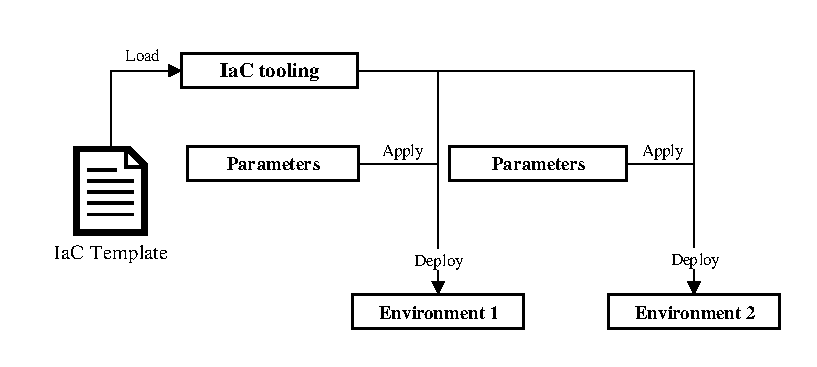
\includegraphics[scale=1]{images/reproduce-infrastructure.pdf}
	\caption{Schema of a parametrized system reproduction}
	\label{fig:reproduce-infrastructure}
\end{figure} 

\subsection{Systems are Disposable}
\label{sec:iac-principles-disposable}
Another benefit of IaC is, that systems are disposable. Disposable means, that systems can be easily destroyed and recreated. Changes made to the templates, describing a system, don't have to be applied on an existing system, but can be applied by destroying and recreating the system. A requirement for a disposable system is, that it is understood, that systems will always change. Other systems, relying on a disposable system, need to address the fact, that the system could change at any time. Systems must not fail, because a disposable system disappears and reappears again because of a redeployment \cite{Morris2016}.

\subsection{Systems are Consistent}
\label{sec:iac-principles-consistency}
Systems managed with IaC are consistent, because they are defined via parametrized templates, and are created by a predefined workflow. All system instances are an instance of the system templates, with the little configuration differences defined by parameters. As long as changes of a system are managed by IaC, the system will stay consistent, and the automation process can be trusted. \\

Listing \vref{src:iac-template-docker-compose} shows an example for an IaC template, which defines a Docker Compose system for hosting a Wildfly server instance. This system can consistently be reproduced on any environment supporting Docker, Docker Compose, and providing values for the defined parameters\cite{Wildfly2017, DockerCompose2018}. \\

\begin{code}
	\yamlFile{\sourceDir/iac-docker-compose.yml}
	\caption{Example for an IaC template of Docker Compose}
	\label{src:iac-template-docker-compose}
\end{code}

\subsection{Actions are Repeatable}
\label{sec:iac-principles-repeatability}
Building reproducible systems means, that any action applied to the system has to be be repeatable. Without repeatability, the automation cannot be trusted and systems wouldn't be reproducible. An instance of a system in one environment has to be equal to any other system instance in any other  environment, except for the configurations defined by parameters. If this is not the case, then a system is not reproducible, because it will have become inconsistent \cite{Morris2016}. \\

IaC is a concept which makes it easy to manage systems in the cloud age. Enterprises can make use of IaC to make their existing systems more reliable, consistent and easier to manage. Nevertheless, before an enterprise can profit from IaC, it has to apply clear structures to their development process, as well as sticking to the automation process provided by the IaC tooling. For experienced administrators, who are used to maintain systems manually, it could be sometimes hard to understand why they are not supposed to perform any actions on the system manually anymore. Being capable to reproduce a system at any time in any environment effortlessly, or applying changes on an existing system in a predefined and consistent manner, makes enterprises very flexible and fast. Enterprises will not have to fear future changes in requirements and technologies of their systems anymore, because they are abstracted from the technologies by the DSL and IaC tool. \\

The following chapter will discuss containerization with Docker, which is very popular tooling for isolating processes on a Linux host. Docker strongly relies on the principle of IaC, and therefore can be seen as a IaC tool for managing isolated processes.    




%\chapter{Containerization with Docker}
\label{cha:containerization-docker}
Docker is a tool for creating, provisioning and interacting with Linux Containers (LXC). LXC are a lightweight version of virtualization, which doesn't have the resource impact of a full virtualization, such as Operating System (OS) virtualization. The differences of LXC and a Virtual Machine (VM) are discussed in Section \vref{sec:docker-virtualization-vs-containerization}. Docker has become very popular over the past years, due to the fact, that it made it possible to easily work with LXC. Docker relies strongly on the principles of IaC which have been discussed in Chapter \vref{cha:iac}. When using Docker, Linux Containers are often referred to as Docker Containers\cite{Docker2018,LXC2018}. \\

Containerization is a key factor when hosting applications in the cloud, because the applications are normally packaged in images and run as containers on the cloud platform. Containerization provides features for a fast, effortless and consistent way of running applications in the cloud, which is discussed in the following section.

\section{The need for Containerization}
\label{sec:docker-need-for-containerization}
Containerization is a key factor for cloud platforms such as PaaS, where each application runs in its own isolated container. A container is an instance of an image, which represents the initial state of an application. A VM represents a full blown OS, whereby the OS provides a kernel, which is emulated by the Hypervisor on the host OS. A Hypervisor is a software, which can create, run, and manage VMs. A container uses the kernel provided by the host OS, and therefore there is no need for a kernel emulation. A container doesn't represent a full blown OS, but still provides features, normally provided by an OS, such a networking and storage\cite{DockerVirtScheepers2014}. \\ 

Containers are faster to create, to deploy, and easier to manage compared to VMs. Nevertheless, cloud platforms use virtualization for managing their infrastructure, whereby the containers run on the provisioned VMs. The usage of containers compared to the usage of VMs can reduce costs for hosting applications. Applications running in containers have less resource impact compared to applications running in VMs, because there is no virtualized OS and no need for kernel emulation. The creation, deployment and startup of containers are faster, because only the isolated process needs to be started and not a full blown OS. Docker is well supported by Integrated Development Environments (IDEs), which provide support for creating Docker Image-Definitions (Dockerfiles) and provisioning of Docker Containers on a local or remote host\cite{DockerFile2018}. \\

When enterprises have applied IaC to their systems, then the next logical step is to apply IaC to their applications as well. Applications running in containers profit from the IaC principles immutability, reproducibility, repeatability, and consistency, which have been discussed in Section \vref{sec:iac-principles}. Docker can be seen as an IaC tool, whereby the Dockerfiles represent the IaC templates and the Docker CLI represents the IaC tool. \\

When using Docker, developers define the process environment for their applications via a Dockerfile, and system administrators provide a VM with the Docker Engine, which is a shift of responsibility. Thus, system administrators have no control about the application environment anymore, which is not considered to be a problem, because the application processes are isolated from other processes, and cannot interfere them. Nevertheless, developers can profit from the deep Linux knowledge of system administrators, to define the Docker Images efficiently, to keep them small and secure. \\

The following sections will give an overview of the Docker technology, its architecture and artifacts.  

\section{Docker}
\label{sec:docker}
Docker is an open source software, which instruments kernel features like LXC. It provides a community edition for free, as well as an enterprise support for production use. The core part of the Docker technology is the Docker Engine, which is discussed in Section \vref{sec:docker-engine}. The Docker Engine is the part of the Docker technology that actually runs the containers. The Docker Images are managed in a so called Docker Registry, which is a repository for Docker Images. The most popular Docker Registry is Docker Hub, which is a free service, where anyone can publish Docker Images\cite{DockerRegistry2018}.

\subsection{Docker Engine}
\label{sec:docker-engine}
Figure \vref{fig:docker-engine} illustrates the Docker Engine architecture hosted on a Linux OS. The Docker Engine is build by layers, whereby each layer communicates with the layer beneath. The Docker Engine was initially designed for LXC exclusively, but has been ported to Windows as well. Docker Images and Docker Containers, which were created for a Windows OS, are not supported on a Linux OS and visa versa, because they use a different OS kernel. The Docker Images and Containers for a Windows OS differ from those for a Linux OS, but the principles of Docker Images and Docker Containers are the same.
\newpage

\begin{figure}[htbp]
	\centering
	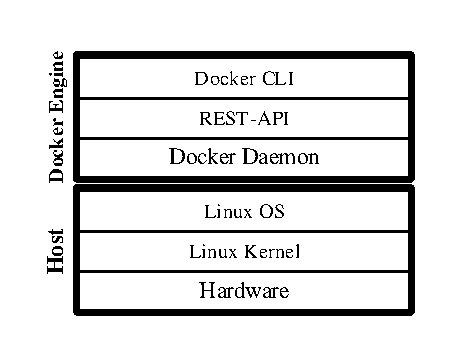
\includegraphics[scale=1]{images/docker-engine.pdf}
	\caption{Docker Engine architecture}
	\label{fig:docker-engine}
\end{figure} 

\mysubsubsection{Docker Daemon}
\label{sec:docker-daemon}
The Docker Daemon represents the background process, which creates, runs and manages the Docker Containers on the Docker Host, and is similar to a VM Hypervisor, but only on process level. The Docker Daemon strongly depends on the kernel of the host OS, therefore incompatibilities could cause the Docker Daemon to fail functioning. The communication with the Docker Daemon is performed via the Docker Engine exposed REST API,  because the Docker Engine is designed as a client server architecture. \\

\mysubsubsection{REST API}
\label{sec:docker-rest-api}
The REST API can be exposed via a Unix socket or a network interface, depending on the configuration of the Docker Daemon. If the REST API is exposed via a network interface, then it is recommended to secure the connection with client certificate authentication. If the Docker Engine and the Docker Client are located on the same host, then commonly the REST API is exposed via a Unix socket and doesn't need any special security. All commands executed via the Docker CLI are actually sent to the Docker Engine via its exposed REST API. \\

\mysubsubsection{Docker Command Line interface}
\label{sec:docker-cli}
The Docker Engine provides a Docker Command-Line-Interface (Docker CLI) for interacting with the Docker Daemon via a Linux shell. The Docker CLI itself is nothing more than a wrapper for the REST API, and communicates with the Docker Daemon via the exposed REST API. This is the most common way to interact with a Docker Daemon. The Docker CLI provides commands for creating container resources such as volumes and networks, managing Docker Images and Containers, and for provisioning the Docker Containers on the Docker Host. \\

\mysubsubsection{Docker Images}
\label{sec:docker-images}
Docker Images are defined via Dockerfiles, which contain instructions how to build the Docker Image. A Docker Image consists of immutable read-only layers, whereby one layer is created for each instruction in the Dockerfile. A layer can contain meta data or a file system state. Docker Images are hierarchical and inherit from another Docker Image, which is then called a base image. Docker Images support only single inheritance and the base image is defined via the \mentionedtext{FROM} instruction, which is the first instruction in the Dockerfile. Docker Images can be identified via their tags, whereby a Docker Image-Tag has the form of \mentionedtext{[url]<namespace>/<name>:<version>} e.g. \mentionedtext{docker.io/library/openjdk:8-alpine}. \\

\mysubsubsection{Docker Containers}
\label{sec:docker-containers}
A Docker Container is an instance of a Docker Image, whereby a new writable layer is appended, which contains all new or modified files. Deleting a Docker Container means, deleting the appended writable layer. Two Docker Containers, created from the same Docker Image, have their own appended writable layer, therefore the Docker Containers are isolated from each other. A Docker Container keeps running as long as the contained foreground process is running. Without a foreground process, the Docker Container stops immediately after the command was executed. The process running in the Docker Container is completely isolated from other processes, and is only allowed to use its assigned resources. \\

\mysubsubsection{Docker Volumes}
\label{sec:docker-volumes}
There are two ways to keep data persistent in Docker Containers. The first one is, to mount a host file system into the Docker Container, whereby the Docker Container depends on the specific host file system. The second one is, to use a Docker Volume, which abstracts the underlying storage type from the Docker Container, and is backed by a storage driver. Cloud storage providers can implement a driver, so that the data, stored in a Docker Volume, is actually kept persistent on a cloud storage. Another advantage of Docker Volume is, that the Docker Volumes can be moved between OS, which support Docker, and allow more detailed configuration.  

\mysubsubsection{Docker Network}
\label{sec:docker-network}
Docker provides networking features, whereby Docker Containers can be connected to each other via a Docker Network. Docker Networks are an abstraction of the actual networks, and are backed by a network driver, which implements the actual network type. The Docker Containers are not aware of the actual network type, the same as they are not aware of the actual storage type with Docker Volumes.

\subsection{Docker Architecture}
\label{sec:docker-architecture}
Figure \vref{fig:docker-architecture} illustrates the Docker architecture, which is a client server architecture. The design as a client server architecture is the reason why the communication to the Docker Daemon is performed via the exposed REST API. The Docker Client communicates with the Docker Daemon via the Docker CLI, whereby the Docker Client can be located on a remote host or on the Docker Host. The Docker Host runs the Docker Engine, which exposes the REST API, the Docker Client connects to. The Docker Engine manages the Docker Images and Docker Containers located on the Docker Host. The Docker Engine can push/pull Docker Images to/from a local/remote Docker Registry.

\begin{figure}[htbp]
	\centering
	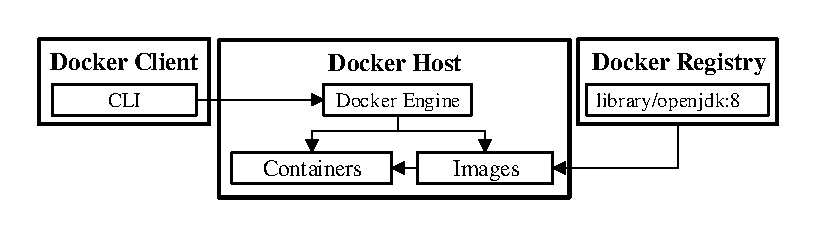
\includegraphics[scale=1]{images/docker-architecture.pdf}
	\caption{Docker architecture}
	\label{fig:docker-architecture}
\end{figure} 

\subsection{Docker Machine}
\label{sec:docker-machine}
The Docker Machine is a tool for managing local or remote Docker Hosts. With Docker Machine, an administrator can manage multiple Docker Hosts via a management server, without the need to connect to the Docker Host via a secure shell (SSH). The Docker Machine CLI provides all necessary commands for managing Docker Hosts. The Docker Engine provisions Docker Containers on a Docker Host and the Docker Machine provisions Docker Hosts on remote Linux hosts. With Docker Machine, a network of Docker Hosts can be managed, which is used by cloud platforms such as Openshift, to manage Docker Engines on the nodes within the Openshift Cluster\cite{DockerMachine2018}.  

\section{Virtualization vs. Containerization}
\label{sec:docker-virtualization-vs-containerization}
Before LXC the industry made use of OS virtualization to isolate their applications. A VM is managed by a Hypervisor, which is a software, which can create, run and manage VMs. The VM provides resources such as network and storage for the application, which is managed by the virtualized OS. Nevertheless, a VM represents a full blown OS, which itself has a resource impact, which adds to the resource impact of the running application. LXC on the other hand is a kernel technology, which provides resources such as network and storage to the application as well, but these resources are managed by the host OS, where the applications are running on.

\subsection{Virtual Machines}
\label{sec:docker-virtual-machines}
A VM is an instance of a Virtual Machine Image (VMI), which is managed by a Virtual Machine Monitor (VMM), which is also referred to as the Hypervisor. The actual difference between a VMM and a Hypervisor is where the software is installed on. If the software is directly installed on the Hardware, then the software is called a Hypervisor, if its installed on the Host OS then its called a VMM. The VM abstracts  an Guest OS from the Host OS, in particular from the underlying hardware. A VM contained Guest OS is not bound to the underlying hardware, because the Hypervisor performs a kernel emulation, which allows to virtualize any Guest OS on any hardware, if the Hypervisor supports it. The following Figure \vref{fig:docker-virtualization-architecture} illustrates the architecture of applications running on a virtualization infrastructure.

\begin{figure}[htbp]
	\centering
	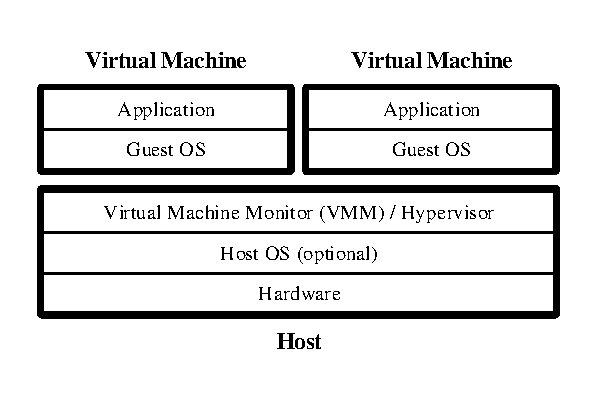
\includegraphics[scale=1]{images/docker-virtualization-architecture.pdf}
	\caption{Architecture of virtualized applications}
	\label{fig:docker-virtualization-architecture}
\end{figure} 

Glauber Costa's started the abstract of his talk at the LinuxCon 2012 with the humorous note \mentionedtext{"I once heard that Hypervisors are the living proof of operating system's incompetence"}. With this note he expressed, that OS weren't able to provide proper isolation for applications, and therefore the industry started to provide an OS instance for each application. This has been overcome with the upcoming of LXC, which provide the proper isolation of applications on the same OS, which made the need for an OS instance for each application obsolete\cite{LxConCosta2012}.

\subsection{Linux Container}
\label{sec:docker-linux-container}
The appearance of LXC has eliminated the shortcoming of the Linux OS, which wasn't able to isolate applications properly, which lead to OS virtualization for application isolation. LXC provide the feature of isolating applications running on the same OS, without the need of a kernel and hardware emulation as it is done with OS virtualization. As illustrated in Figure \vref{fig:docker-container-architecture}, the application process, binaries, and libraries are bundled into the container, and are isolated from other containers. Each container gets a portion of the global resources such as CPU cycles and memory assigned, and cannot consume more as it has been assigned to. Without LXC it is possible that one process takes over all available system resources, whereby other processes would starve.

\begin{figure}[htbp]
	\centering
	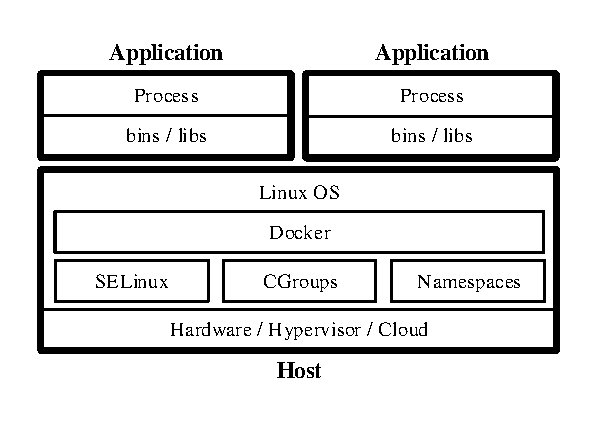
\includegraphics[scale=1]{images/docker-containerized-architecture.pdf}
	\caption{Architecture of containerized applications}
	\label{fig:docker-container-architecture}
\end{figure} 

The following sections will discuss the two most important kernel features for LXC, Cgroups and Namespaces, which provide resource control and isolation. 

\mysubsubsection{Cgroups}
Cgroups stands for control groups, and Cgroups provide the ability to aggregate processes, their child processes and threads, to groups, which are managed in a tree structure. Each group gets a portion of the global resources such as CPU cycles or memory assigned, whereby it is guaranteed, that a group and its managed processes cannot consume more resources as the group has been assigned to. Each process running in a container is assigned to a group, whereby a process cannot steal resources from another process anymore, because the resource assignments of a group, managed by Cgroups, prevents this from happening\cite{KernelCGroupsV12018, KernelCGroupV22015, IntelLXCHyperVisor2014}. \\

\mysubsubsection{Namepsaces}
Cgroups manage how many resources can be used by processes in a group, and Namespaces manage the view of the system to processes. A container is managed in its own namespace, and therefore the container has a limited view of the system, such as networks and process ids (PIDs). Namespaces are a fundamental concept of LXC, and Namespaces provide the isolation between containers\cite{LinuxNamespaces2018, IntelLXCHyperVisor2014}. \\

The following chapter will discuss Kubernetes, which is an orchestrator for Docker Containers, and allows to manage Docker Containers in a clustered environment. 
 


%\chapter{Container as a Service with Kubernetes}
\label{cha:caas}
Container as a Service (CaaS) is a term introduced by cloud providers, which provide a cloud based on demand container environment. But CaaS is more then just an on demand container environment like Docker, it provides orchestration and monitoring tooling for containers. Additionally, CaaS is considered to be a model for IT organizations and developers, how they can ship and run their applications anywhere. There are multiple CaaS providers on the market, but the most popular CaaS providers are Azure Container Service, Amazon Elastic Container Service for Kubernetes (Amazon EKS), and Google Kubernetes Engine, whereby they bring in their own flavor of CaaS, but all of them use Kubernetes beneath\cite{CNCFKubernetes2018, MicrosoftAzureAKS2018, AmazonWebServicesEKS2018, GoogleCloudKE2018}. \\

Kubernetes is a container orchestration platform for automating deployments, scaling, and operation of containers across a Kubernetes Cluster. Kubernetes has been invented by Google, is open source since 2015, and managed by the Cloud Native Computing Foundation (CNCF), whereby CNCF is under the umbrella of the Linux Foundation. Kubernetes has become the most popular container orchestration platform on the market and is used by many CaaS and PaaS providers\cite{CNCF2018}.

\section{The need for Container as a Service}
\label{sec:caas-need-for-caas}
Enterprises and developers face the need to dynamically adapt to workloads and to roll out new version of their services fast, and without any downtime. Applying dynamically to workloads requires a dynamic infrastructure, which is capable of scaling up when the workload increases, and scaling down when the workload decreases, which is non-trivial to be handled manually. Rolling out new versions without downtime require a well defined workflow, which ensures a well defined roll out behavior. For such uses cases, a CaaS platform like Kubernetes can be used. Kubernetes makes it possible to effortlessly manage complex service infrastructures, service scaling, and the roll out of services. Thus, complex service infrastructures become simple to implement and manage.
\newpage

Kubernetes provides a DSL, which allows to specify the desired state of the Kubernetes Cluster, as well as a automation tooling to interact with the Kubernetes Cluster. Kubernetes automatically ensures that the state of the Kubernetes Cluster meets its specification. Thus, the developers have only the need to specify the desired state of their Kubernetes Cluster. Kubernetes provides enterprises a platform for their services, which is effortlessly to specify and maintain via templates and the provided automation tooling, which makes Kubernetes an IaC tool as well, as discussed in Chapter \vref{cha:iac}. This makes it easy to modify the infrastructure at any time, which allows enterprises to apply to new requirements fast.

\section{Kubernetes}
\label{sec:caas-kubernetes}
Kubernetes is a CaaS platform to orchestrate containers in a cluster, whereby the Kubernetes Cluster nodes can be located in the cloud or in a dedicated data center. Kubernetes is designed as a client server architecture and a master slave architecture. At least one node in the Kubernetes Cluster acts as the Kubernetes Master, which is discussed in Section \vref{sec:caas-kubernetes-master}, and the other nodes in the Kubernetes Cluster act as the Kubernetes Workers, which are discussed in Section \vref{sec:caas-kubernetes-worker}. The Figure \ref{fig:kubernetes-cluster-architecture} illustrates the architecture of a Kubernetes Cluster.

\begin{figure}[htbp]
	\centering
	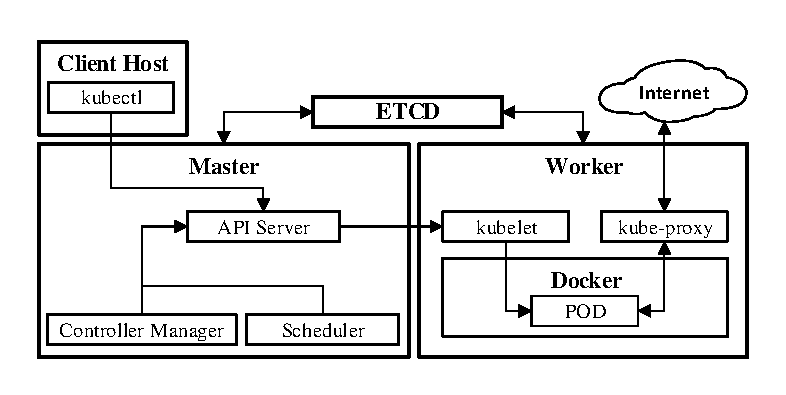
\includegraphics[scale=1]{images/kubernetes-cluster-architecture.pdf}
	\caption{Architecture of a Kubernetes Cluster}
	\label{fig:kubernetes-cluster-architecture}
\end{figure} 

\subsection{Kubernetes Objects}
\label{sec:caas-kubernetes-objects}
Kubernetes Objects are persistent objects in the Kubernetes System, and the Kubernetes Objects describe the state of the Kubernetes Cluster. The Kubernetes Cluster ensures that the state of the cluster meets the state specified by the Kubernetes Objects. The developers don't have to manually perform actions in the Kubernetes Cluster, they just have to modify the state represented by the Kubernetes Objects, and the Kubernetes Clusters itself will ensure that the modified state is applied on the Kubernetes Cluster. The following sections will briefly introduce some of the common used Kubernetes Objects. The overview of all Kubernetes Objects is covered by the Kubernetes API reference documentation\cite{CNCFKubernetesAPI2018}. 

\mysubsubsection{Pod}
A Pod is a group of one or more containers, which are managed together, and therefore share the same life-cycle. A Pod specification contains the specification for each container in the group. All of the containers of a Pod are always located on the same Kubernetes Worker, and will be deployed, started, and stopped as a single unit. In a pre-container world, all of the applications represented by the containers would have been hosted on the same physical machine. A Pod allows to bundle containers together, whereby the containers in a single Pod represent one instance of an  application\cite{CNCFKubernetesPods2018}. 

\mysubsubsection{Service}
A service is an abstraction, which defines a set of Pods and policies how to access them. The connection to the Pod, via the service abstraction, is handled by the Kubernetes Proxy. The service abstraction is necessary, because a Pod can be located on any Kubernetes Worker within the Kubernetes Cluster, and the Pod will therefore get a random IP assigned, which makes it impossible to address the Pod directly. If multiple replicas of a Pod are running, then the service will load balance the request between the Pods of the replica set, depending on the chosen algorithm\cite{CNCFKubernetesServices2018}.

\mysubsubsection{Secret}
A secret is an abstraction to manage sensitive configuration data, which can be consumed by containers. A secret holds a set of key value pairs, which represents the sensitive configuration data, and can be referenced by its name. A referenced secret can be injected into the container, either as a environment variable or a file. If the secret is injected as a file, then the filename represents the secret key and the file content represents the secret value. Developers reference secrets in the Pod specifications by their name, and only the referencing containers can access the injected sensitive configuration data the secret holds\cite{CNCFKubernetesSecrets2018}. 

\mysubsubsection{ConfigMap}
A configuration map works the same way as secrets, but is intended to hold non sensitive configuration data\cite{CNCFKubernetesConfigMap2018}.

\subsection{Kubernetes Master}
\label{sec:caas-kubernetes-master}
The Kubernetes Master is the master node in the Kubernetes Cluster, and is responsible for managing the Kubernetes Workers and Pods running on them. The Kubernetes Master exposes a REST API, via clients can interact with the Kubernetes Cluster. The node hosting the Kubernetes Master should be exclusively for the Kubernetes Master. The following sections briefly introduce the Kubernetes Master-Components, which are responsible for managing the Kubernetes Cluster\cite{CNCFKubernetesComponents2018}.

\mysubsubsection{Kubernetes CLI (kubectl)}
Kubectl is the CLI of Kubernetes, which provides an interface to manage the Kubernetes Cluster, and the Pods running on the Kubernetes Workers. Kubectl is similar to the Docker CLI, but does not support direct interacting with Docker. Kubectl interacts with the Kubernetes Cluster via the REST API exposed by the Kubernetes Master API-Server. Kubectl can be used from any client machine, which can connect to the cluster without any special setup.

\mysubsubsection{Distributed Key-Value Store (etcd)}
Etcd is a distributed key-value store, and provides a reliable way for sharing data within a cluster. It is the key component for the communication between the Kubernetes Masters and the Kubernetes Workers. The Kubernetes Master provides configuration for the Kubernetes Workers, and the Kubernetes Workers provide state information for the Kubernetes Master\cite{CoreOSETCD2018}.

\mysubsubsection{Kubernetes API-Server (kube-apiserver)}
The Kubernetes API-Server exposes the REST API for interacting with the Kubernetes Cluster, and is located on the Kubernetes Master. It represents the front-end of the Kubernetes Cluster and provides all necessary API to manage the Kubernetes Cluster, and the Kubernetes Objects.

\mysubsubsection{Kubernetes Scheduler (kube-scheduler)}
The Kubernetes Scheduler watches the Kubernetes Cluster for newly created Pods and assigns the Pods to a Kubernetes Worker. The Kubernetes Scheduler decides which Kubernetes Worker is suitable for the Pod. Multiple factors are taken into account for scheduling decisions such as, individual specifications, resource requirements, available resources, and hardware/policy/software constraints.

\mysubsubsection{Kubernetes Controller Manager (kube-controller-manager)}
The Kubernetes Controller Manager is responsible for managing the different controllers. A Kubernetes Controller is running in a loop and ensures that the state of the system is valid, depending on the controller type. For instance, the replication controller ensures the correct number of Pods for each replication controller object within the Kubernetes Cluster. Kubernetes provides a set of controllers such as, a replication controller, node controller, endpoint controller, and service account controller.

\subsection{Kubernetes Worker}
\label{sec:caas-kubernetes-worker}
The Kubernetes Worker is a node within the Kubernetes Cluster, which acts as the slave node, which runs the Pods, and is managed by the Kubernetes Master. The Kubernetes Worker can be a VM or a physical machine, depending on the Kubernetes Cluster setup. It contains the Kubernetes Runtime-Environment and used container runtime. The following sections briefly introduce the Kubernetes Worker-Components, which are responsible for running the Pods on the Kubernetes Worker\cite{CNCFKubernetesComponents2018}. 

\mysubsubsection{Kubernetes Agent (kubelet)}
The Kubernetes Agent is a process, running on the Kubernetes Worker, which interacts with the Kubernetes Master via its exposed REST API. The Kubernetes Agent ensures, that the containers are running in a Pod, as specified by the provided Pod specifications. The Pod specifications can be provided by a file in a specific directory, which gets periodically checked, or via the Kubernetes API-Server.

\mysubsubsection{Kubernetes Network-Proxy (kube-proxy)}
The Kubernetes Network-Proxy manages the networks defined by the specifications, and reflects the services, which are bound to a Pod. It can perform simple TCP and UDP forwarding, and can be connected to multiple back-ends. Any communication of a Pod to another Pod or to an external network is handled by the Kubernetes Network-Proxy. 

\mysubsubsection{Container Runtime}
The container runtime is the software responsible for running the containers on the Kubernetes Worker. Kubernetes supports multiple container runtimes, but mostly  Docker is used, which has been discussed in Chapter \vref{cha:containerization-docker}. \\

Kubernetes provides all features to implement a dynamic scalable service infrastructure such as, workflows for rolling out services, replica management, or secret and configuration management. Kubernetes is on top of the container runtime such as Docker, and provides orchestration tooling, necessary to run large scale containerized service infrastructures. Nevertheless, sometimes a pure container orchestration platform like Kubernetes is not enough, which for instances doesn't provides features for setting up a complete release workflow. This can be overcome with the usage of PaaS platforms like Openshift, which will be discussed in the following chapter.

%\chapter{Platform as a Service with Openshift}
\label{cha:paas}
Platform as a Service (PaaS) is a cloud service, which provides an on demand platform for building, deploying and running containerized applications in the cloud. PaaS can be seen as an enhancement of CaaS, which has been discussed in Chapter \vref{cha:caas}. A PaaS platform does not only provide a container runtime for running containers in the cloud, but also tooling for building, deploying and monitoring of containerized applications, as well as security mechanisms for securing those applications. There are multiple PaaS providers on the market but the most popular PaaS providers are RedHat Openshift Online, Microsoft Azure Cloud Services, Google App Engine and AWS Elastic Beanstalk. They all bring in their own flavor of PaaS but they all provide similar features expected from a PaaS platform\cite{OpenshiftOnline2018, MicrosoftAzueCloudServices2018, GoogleCloudAE2018, AmazonWebServicesEBT2018}. \\

PaaS providers usually provide templates for the major programming languages, application servers, as well as integrations to other cloud services. External cloud services of the same vendor are usually better supported than cloud services of other vendors. This is normal, because cloud providers want the customers to use their services over the services of the competition. What all PaaS providers have in common, is the consumption based pricing model, whereby only the consumed physical resources have to be paid for, and the ability to scale with the workload. \\ 

IPaaS can be seen as an enhancement of PaaS, which provides special features for implementing an ESB, which is discussed in Chapter \vref{cha:esb}. IPaaS enhances an ordinary PaaS platform by providing tooling for integrating external services effortlessly via a low/no code platform, whereby service integrations can be defined via an UI, rather then by implementing source code. Red Hat Fuse 7 is an example for an IPaaS platform, which will replace JBoss Fuse 6.x in the near future\cite{Fuse72018, iPaaSP12015, iPaaSP22015}. \\

Openshift Origin is an open source PaaS platform, which has been released in April 2012 and is the upstream project for Red Hat Openshift Enterprise. Before Openshift 3 (Jun 2013), Openshift used its own container runtime and orchestration tooling, which since Openshift 3, have been replaced by Docker and Kubernetes, because of its popularity and general availability. Openshift is the only major PaaS platform of the previously noted ones, which can be self hosted or hosted by a local provider. The other major PaaS providers, such as Microsoft Azure, are only available as a cloud service, which are hosted in the vendors data centers\cite{OpenshiftOriginGithub2018}.

\section{The need for Platform as a Service}
\label{sec:paas-need-for-paas}
PaaS platforms like Openshift are based on a CaaS platform, and enhance CaaS by providing a web console, and templates, which allow to define all necessary resources for a service, as well as its release behavior. An instance of a service can be created via the web console, whereby only the required values for the exposed parameters of the template have to be provided. CaaS alone is suitable if its used by developers, but is not suitable for persons without any deep knowledge of containerization and container orchestration. This is where PaaS platforms come into place. Developers specify templates for the provided services, which specify the necessary service resources, and non-developers create a service instance via the web console. The PaaS platform takes the template and provided template parameter values and provisions the service for the user. \\

Enterprises can profit from PaaS platforms, by defining templates for services they provide for their departments, partners or customers, who can create an instance of a service on demand, and destroy it if not needed anymore. PaaS platforms provide a self service console, where services can be created, managed and destroyed effortlessly, without the need to understand the underlying platform. The self service console could be implemented by enterprises for their specific use cases, whereby the custom self service console interacts with PaaS platform via its exposed REST API. \\

PaaS platforms like Openshift usually provide an integration in a Continuous Integration / Continuous Deployment (CI/CD) workflow, which allows to automatically build and deploy new service releases on the PaaS platform in a predefined manner. Therefore, the PaaS platforms are integrated in the whole software life-cycle. This decreases the effort of the developers to interact with the cloud platform and provides additional automation.
 
\section{Openshift}
\label{sec:paas-openshift}
Openshift is a open source PaaS platform, which uses Docker as the container runtime and Kubernetes for the container orchestration. Openshift is designed as a client server architecture and a master slave architecture, the same way as Kubernetes, which has been discussed in Section \vref{sec:caas-kubernetes}. An Openshift Cluster can contain multiple Kubernetes Clusters, which are managed by the Openshift Master. Openshift introduces the concept of a project, which is actually a Kubernetes Namespace, whereby a project is completely isolated from other projects. Figure \vref{fig:paas-openshift-kubernetes-cluster-architecture} illustrates the architecture of an Openshift Cluster\cite{OpenshiftDeepDive2014, OpenshiftCoreConcepts2018}.

\begin{figure}
	\centering
	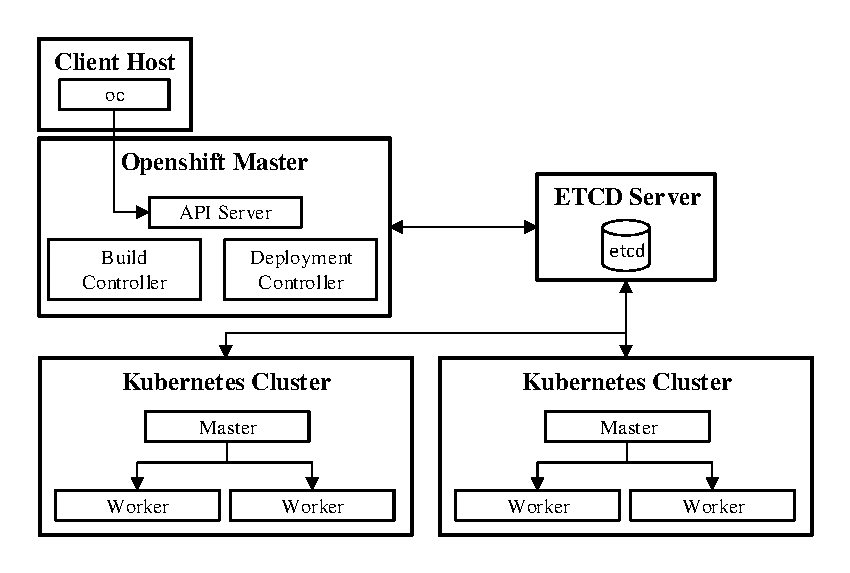
\includegraphics[scale=1]{images/openshift-kubernetes-cluster-architecture.pdf}
	\caption{Architecture of an Openshift Cluster}
	\label{fig:paas-openshift-kubernetes-cluster-architecture}
\end{figure} 

\subsection{Openshift Master}
\label{sec:paas-openshift-master}
The Openshift Maser manages the Kubernetes Master of the Kubernetes Clusters the Openshift Cluster contains. The Openshift Master exposes a REST API via the clients can interact with the Openshift Cluster. Openshift is placed on top of Kubernetes, whereby the Openshift Master node acts similar as a Kubernetes Master node, which has been discussed in Section \vref{sec:caas-kubernetes-master}. Additionally, Openshift provides features, which are not provided by Kubernetes, such as, a role and group based security model for isolating the Kubernetes Namespaces via Openshift Projects, and controllers for managing the additional Openshift Objects. The following Section will discuss the Openshift Project, which is one of the new features provided by Openshift.

\subsection{Openshift Project}
\label{sec:paas-openshift-project}
An Openshift Project represents a Kubernetes Namespace, where all resources of an Openshift Project are located. An Openshift Project provides the isolation and security for a Kubernetes Namespace, which are not provided by Kubernetes itself. Figure \vref{fig:paas-openshift-project-architecture} illustrates the Openshift Project architecture, its contained objects, and their dependencies to each other. The bold marked objects represent the new objects, which were introduced by Openshift.
\newpage

\begin{figure}[htbp]
	\centering
	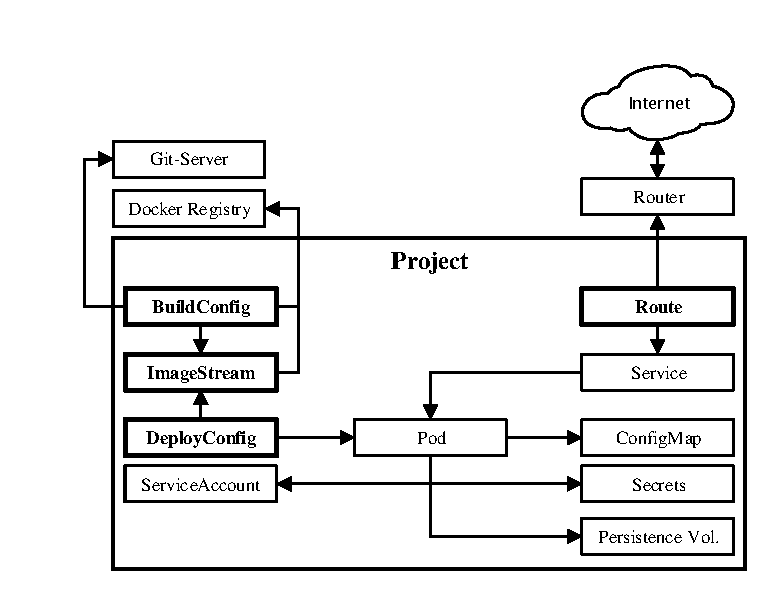
\includegraphics[scale=1]{images/openshift-project-architecture.pdf}
	\caption{Architecture of an Openshift Project}
	\label{fig:paas-openshift-project-architecture}
\end{figure} 

Openshift Objects are persistent objects in the Openshift System, and the Openshift Objects describe the state of the Openshift Cluster. This behavior has been inherited from the underlying Kubernetes System, as discussed in Section \vref{sec:caas-kubernetes-objects}. The following sections briefly introduce the new objects provided by Openshift. 

\mysubsubsection{Openshift BuildConfig}
An Openshift BuildConfig specifies the way how a Docker Image is built on the Openshift Cluster, whereby the built Docker Image is pushed into the Openshift internal Docker Registry. An Openshift BuildConfig supports the following listed strategies:
\begin{itemize}
	\item The \emph{Source-to-Image (S2I)} strategy, is the build strategy, which builds a Docker Image from application source code with a so called builder image.
	\item The \emph{Docker} strategy, is the build strategy, which builds a Docker Image from a Dockerfile.
	\item The \emph{Custom} strategy, is the build strategy, which builds a Docker Image with a custom implemented build mechanism.
	\item The \emph{Pipeline} strategy, is the build strategy, which performs a Jenkins Pipeline build on a Jenkins build server.
\end{itemize}

The sources for a build are provided via a git repository, and an Openshift BuildConfig can be triggered via a web hook by an external git server\cite{S2I2018, OpenshiftBuildStrategies2018}. 

\mysubsubsection{Openshift ImageStream}
An Openshift Image Stream and its Image Stream-Tags are an abstraction of the actual used Docker Image, and an Image Stream uses the same naming convention as Docker Tags (E.g \mentionedtext{myproject/app:1.0}), whereby
\begin{itemize}
	\item \mentionedtext{myproject} represents the Image Stream namespace,
	\item \mentionedtext{app} represents the Image Stream and
	\item \mentionedtext{1.0} represents the Image Stream-Tag.
\end{itemize}
An Image Stream-Tag references a Docker Image instance by its Docker Image-Id, because a Docker Image-Id always references the same Docker Image instance, whereby a Docker Image-Tag can reference different Docker Image instances. Once the Docker Image has been imported, it will not be automatically pulled again, unless the Image Stream-Tag is named \mentionedtext{latest}. \\

A Docker Image can be updated in a Docker Registry, which would break the consistency principle, because it wouldn't be the same Docker Image as used before the update. An Image Stream, in particular the Image Stream-Tag, avoids this by referencing the Docker Image-Id, which makes a used Docker Image immutable within an Openshift Project, unless the name \mentionedtext{latest} is used for the Image Stream-Tag\cite{OpenshiftBuildAndImageStreams2018}.

\mysubsubsection{Openshift DeployConfig}
An Openshift DeployConfig specifies how a deployment of a Pod has to be performed. An Openshift DeployConfig allows to specify the Kubernetes life-cycle hooks pre-hook or post-hook, which are used to configure the deployed Pod before its process has started (pre-hook) or after its process has started and is ready (post-hook). An Openshift DeployConfig supports the following listed deployment strategies\cite{OpenshiftDeployments2018}:
\begin{itemize}
	\item The \emph{Rolling} strategy, is the deployment strategy, which waits for the new deployment to be ready before the old deployment gets removed.
	\item The \emph{Recreate} strategy, is the deployment strategy, which removes the old deployment when the new deployment gets started.
	\item The \emph{Custom} strategy, is the deployment strategy, which performs the deployment by a custom implementation.
\end{itemize}

\mysubsubsection{Route}
An Openshift Route exposes a Service with a host name to an external network, so that it can be reached by its host name from outside the Openshift Project. The Route is deployed on an Openshift Router, which performs the routing between the external network and the connected Openshift Service. A Route can be secured with TLS, whereby the certificates of the Openshift Cluster can be used, or the certificate can be directly defined on the Openshift Route. \\

The following section will discuss the Enterprise Service Bus, which will be implemented by the prototype and hosted on an Openshift Cluster.
%\chapter{Enterprise Service Bus}
\label{cha:esb}
An Enterprise Service Bus (ESB) is a architectural pattern of the Software Oriented Architecture (SOA) Patterns, which describes a distributed computing architecture, whereby distributed services are interacting with each other via a bus system. An ESB in the industry is mostly taken as a third party middleware, which provides features for implementing integrations with the Enterprise Integration (EI) Patterns. Enterprises use third party middleware like JBoss Fuse for implementing integration services, which integrate external or internal services. JBoss Fuse is based on JBoss EAP, and bundles common frameworks used for integrations such as Camel, and is responsible for orchestration and mediation of the services. Camel provides API and implementations for the EI patterns and is widely used in the industry when it comes to integrate services\cite{CamelIA2018, Camel2015}. \\

The integration of external as well as internal services has become more important over time, especially with the appearance of cloud services like PaaS. Common ESB middleware on the market usually define the ESB as a single application, which contains all integration services, whereby all integration services share the same life-cycle. A single application representing an ESB, is contrary to its definition as a distributed architectural model, but has the advantage, that the ESB application is compiled at once, and therefore its contained services have to be consistent. Over time, the handling of the single ESB application will become inconvenient and complex, which is a common problem for a monolithic application.  \\

The increasing need for flexibility and shorter response times drives enterprises to split up their teams and integrations. This leads to separated services, which are managed as microservices, which have their own life-cycle. Decoupling of teams leads to decoupling of services, where the services need to provide a well defined and well managed public API\cite{Camel2015, RedHatAgileIntegration2017, EIP}.

\section{The need for an Enterprise Service Bus}
\label{sec:esb-need-for-esb}
Enterprises need an ESB to provide integrations between internal and external services or both, whereby the integrations are meant to provide a business value for the enterprise. An integration of an external service could enhance the reach of a customer, who now could be able to consume external partner services via the enterprise provided infrastructure or product. In the digital age, it is normal to consume a digital service like Netflix, which provides a video on demand service. Thus, integrations, an enterprise has to provide and maintain, will become more over time.

\section{Architecture}
\label{sec:esb-architecture}
Figure \vref{fig:esb-simple-architecture} illustrates the conceptional architecture of an ESB, which orchestrates and mediates integration services. A service can act either as a producer service, which gets accessed by clients, or can act as a consumer service, which acts as the client for a producer service. The ESB is responsible for orchestration, mediation, security, transformation, routing, and service discovery, whereby these aspects are covered by an ESB middleware provided frameworks and libraries. Additionally, an ESB middleware provides libraries, which help to implement Service Components under consideration of the SOA and EI Patterns\cite{EsbSoa2018, MediationESB2005}.

\begin{figure}[htbp]
	\centering
	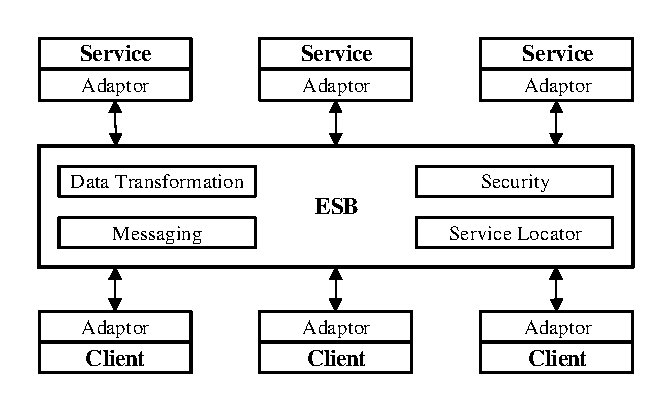
\includegraphics[scale=1]{images/esb-simple-architecture.pdf}
	\caption{Architecture of an ESB}
	\label{fig:esb-simple-architecture}
\end{figure} 

Figure \vref{fig:esb-bidirectional-integration} illustrates a bi-directional integration of services between two partner enterprises, whereby each integrated service is allowed to be consumed by the partner's customers, but only if the service is accessed via the partner's infrastructure. The ESB of the enterprises integrate the partner's provided services into their service domain, which can be accessed by their customers. For instance, an IP-TV provider can be integrated by an Internet Service Provider (ISP), to provide Internet TV for their customers.
\newpage 

\begin{figure}[htbp]
	\centering
	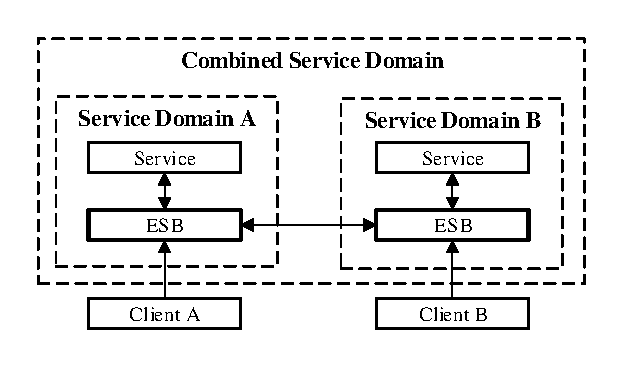
\includegraphics[scale=1]{images/esb-bidirectional-integration.pdf}
	\caption{Architecture of a bi-directional enterprise integration}
	\label{fig:esb-bidirectional-integration}
\end{figure} 

\section{Enterprise Service Bus with EAP}
\label{sec:esb-as-software}
An ESB is an architectural model for a distributed system, and has been implemented in software to provide an integration platform to developers, so that they can implement services under the consideration of the EI patterns. Before the appearance of cloud services like PaaS, ESB implementations used existing platforms such as JBoss EAP, OSGI or Karaf for the service orchestration and mediation. In case of JBoss EAP, the platform provides all libraries and frameworks developers need for implementing a service. Commonly, the services are managed within a single application, which represents the ESB application. This is a monolithic approach of organizing services, but has the advantage that the management of the services is easier, because the source code is not separated. Figure \vref{fig:esb-software-architecture} illustrates the monolithic organization of the services within a single ESB application, which is hosted on JBoss EAP.

\begin{figure}[htbp]
	\centering
	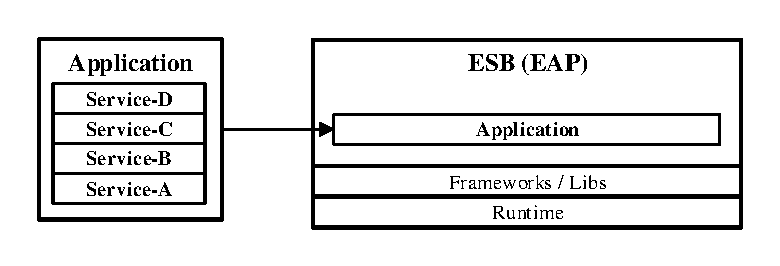
\includegraphics[scale=1]{images/esb-software-architecture.pdf}
	\caption{Monolithic ESB application}
	\label{fig:esb-software-architecture}
\end{figure} 
\ \newpage

Figure \vref{fig:esb-software-architecture} was called an ESB, but is actually not one, because the services are not distributed. Nevertheless, the industry calls such installations an ESB. The services of such an ESB application are implemented separately, but still managed within a single code base, and communicate with each other like they where on a bus system. JBoss EAP proxies the requests between the services, and therefore acts more like a message broker of an Hub and Spoke architecture, rather than acting as a bus system. The Hub and Spoke architecture was introduced, due the fact, that the count of edges of a fully connected graph requires $n / 2 * (n -1)$ edges, whereby the count of edges grows with the square of the count of nodes. A node in the graph represents a service, and an edge in the graph represents the connection between two services\cite{EIP,HubAndSpoke2003}. \\

With the appearance of cloud services such as PaaS, the PaaS platform can now take over the mediation, and security aspects of an ESB. The services can be completely separated and decoupled from each other, designed as microservices with their own life-cycle, and be managed by the cloud service. Additionally, the services are hosted in a clustered infrastructure, which allows them to be distributed among multiple nodes. The new term for this kind of ESB is IPaaS, whereby the ESB is represented by an PaaS platform such as Openshift, which provides additional tooling for implementing integration  services\cite{iPaaSP12015, iPaaSP22015}.

\section{Enterprise Service Bus with Openshift}
\label{sec:esb-as-cloud}
With the appearance and general availability of cloud services like PaaS, it is now possible to move an ESB into the cloud, whereby the cloud service takes over some aspects of the ESB middleware such as mediation and security. Openshift performs mediation via the Openshift Service abstraction, whereby multiple service instances can be present behind the Openshift Service, and the security is applied by isolating the Openshift Projects, and making services only accessible within an Openshift Project, or via an Openshift Route. The service orchestration is not needed anymore, because the services are now microservices, which need service choreography. The main difference between service orchestration and service choreography is, that the service orchestration has a local point of view and a central orchestrator component, whereby the service choreography has a global point of view and no central orchestrator component\cite{Richards2015}. \\

A main problem of existing monolithic ESB applications is the fact, that all services are managed within a single application, with one release version, and a shared life-cycle. If the ESB is represented by a cloud service, the services have to be implemented as separated services, which forces developers to separate their services into separate code bases, and to provide a proper designed and managed public API for their services. Figure \vref{fig:esb-cloud-architecture} illustrates the services of an ESB application, which runs on Openshift. \\

As discussed in the introduction of this chapter, enterprises need to separate their integrations and teams, to be faster and more responsive to business changes. Therefore, the microservice architecture, which is necessary when the ESB is represented by a cloud service, can help enterprises to become more flexible.

\begin{figure}[htbp]
	\centering
	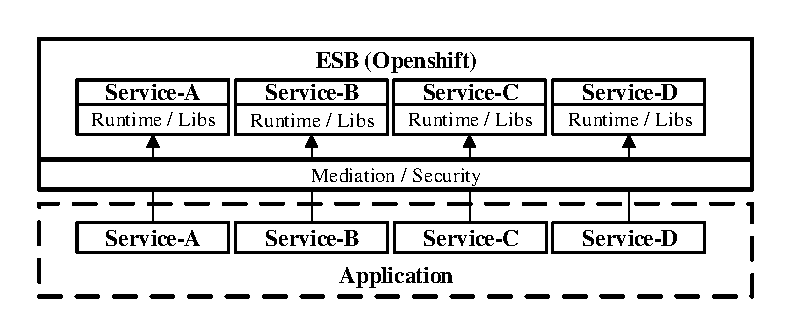
\includegraphics[scale=1]{images/esb-cloud-architecture.pdf}
	\caption{ESB application with microservices}
	\label{fig:esb-cloud-architecture}
\end{figure} 

\section{Service Integration Example}
\label{sec:esb-integration-example}
This section will discuss an example of a service integration, and how it would have been designed as part of a monolithic ESB application with JBoss Fuse based on JBoss EAP. The integration discussed in this chapter will be the base for the prototype of this thesis, which is specified in Chapter \vref{cha:esboc}. Figure \vref{fig:esb-design-services} illustrates the integration example, contained services, and involved service domains. The integration service integrates an external database with an internal application, which is consumed by a public client. How the database is allowed to be accessed is implemented in the integration service, which is the only service allowed to communicate with the external located database.

\begin{figure}[htbp]
	\centering
	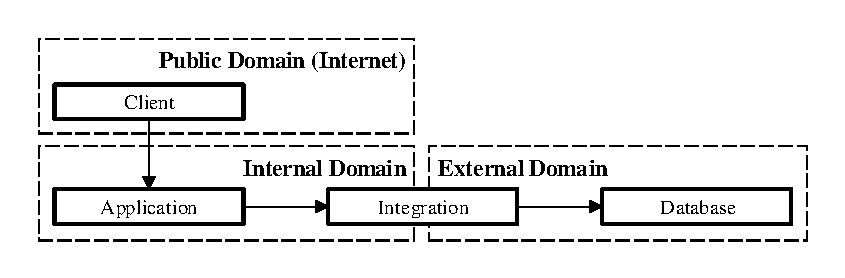
\includegraphics[scale=1]{images/esb-integration-example.pdf}
	\caption{Integration example service domains}
	\label{fig:esb-design-services}
\end{figure}
\ \newpage

Figure \vref{fig:esb-design-sca} illustrates the design of the integration in an monolithic ESB application with JBoss Fuse based on JBoss EAP and Switchyard, which provides an API for implementing a Service Component Architecture (SCA). A service within the ESB application is represented by a service component, which exposes consumable resources (Service), and calls other services (Reference)\cite{Switchyard}. 

\begin{figure}[htbp]
	\centering
	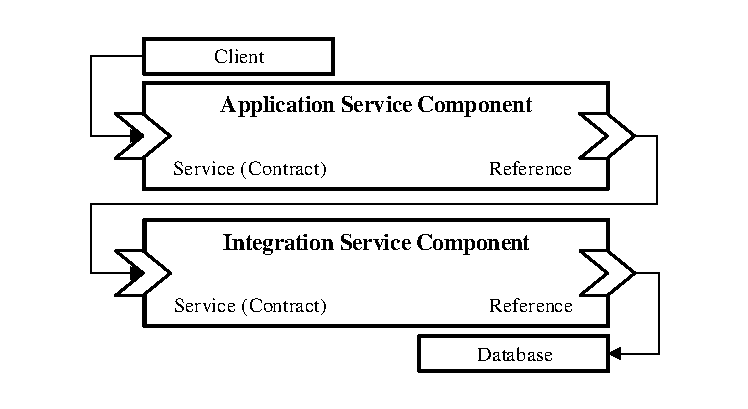
\includegraphics[scale=1]{images/esb-sca-example.pdf}
	\caption{Integration with SCA}
	\label{fig:esb-design-sca}
\end{figure}
  
ESB middleware, such as JBoss Fuse, provides frameworks and libraries, which implement the SCA patterns and provide a lightweight way of implementing service components. The service component orchestration, mediation, and security is performed by the ESB middleware. Additionally, the ESB middleware provides bindings for commonly used technologies such as REST or SOAP, which can be applied to services and references. Thus, the developers don't have to setup for instance a REST Server or REST Client anymore, but only need to provide the service contract and connection settings\cite{MicroSoa2008, Richards2015}.\\

The following chapter will specify the prototype based on the introduced example integration, and will show that an ESB can be implemented on Openshift.
%\chapter{Design ESB in Openshift}
\label{cha:esboc}
In this chapter, the ESB example integration of Section \vref{sec:esb-integration-example} will be designed as microservices, which can run on a Openshift Cluster. An Openshift Project will act as the ESB, which will provide the mediation, security, configurations and secrets for the services. The concrete functionality of the services is considered to be not important. The goal is to redesign the service components of Figure \vref{fig:esb-design-sca} as microservices, and to design the Openshift Project, which will host the services and act as the ESB. \\

As discussed in Chapter \vref{cha:esb}, an ESB is a distributed architectural model, whereby services act as a consumer or producer. These services provide a business value for an enterprise in form of an integration of an internal or external service. There are multiple providers of ESB middleware like JBoss Fuse, which provide tooling for implementing service components running on the ESB middleware. The prototype will illustrate that SOA service components can be implemented as microservices, whereby features provided by the ESB middleware, such as bindings, will have to be replaced by other implementations.

\section{Microservice Architecture}
Figure \vref{fig:esboc-design-services} illustrates the microservice architecture of the example integration of Figure \vref{fig:esb-design-sca}. Conceptually, the transformation of a service component to a microservice is easy, because a service component and a microservice act very similar. Compared to a service component of an ESB middleware, a microservice is completely separated from the other services, brings in its own libraries, and runs in its own runtime environment. From the implementation point of view, the microservices need to provide an runtime environment, which was previously provided by the ESB middleware. Therefore, that the microservices are completely separated, the access of other services is not mediated as usual anymore, because the communication is now performed via standard protocols like HTTP(S). In a monolithic ESB application, running on JBoss EAP, every service component is accessed via a reference, whereby the reference proxies the request directly to the service, which is running in the same runtime environment. With microservices, running in their own runtime environment, it is not possible to access the service instance directly anymore. Only communication via standard protocols, such as HTTP(S), is supported.

\begin{figure}[htbp]
	\centering
	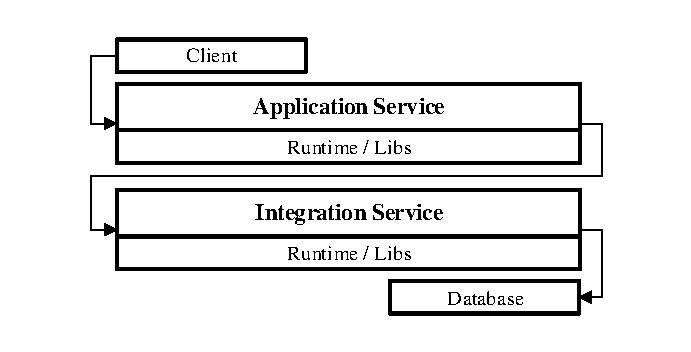
\includegraphics[scale=1]{images/esboc-design-microservice.pdf}
	\caption{Integration with microservices}
	\label{fig:esboc-design-services}
\end{figure}

\section{Microservice Aspects}
\label{sec:esboc-aspects}
This section will discuss the necessary aspects of microservices, which will ensure, that the services are properly implemented, and can effortlessly be managed. Especially the monitoring of the services becomes very important, when moving from a conventional monolithic ESB application, like an application running on JBoss Fuse, to a microservice architecture based ESB application. Services running as microservices on Openshift, are running in their own runtime environment, and therefore cannot share any runtime resources. \\

Figure \vref{fig:esboc-aspects} illustrates the hierarchy of the microservice aspects, which will ensure that the implemented services are
\begin{itemize}
	\item secure,
	\item configurable for multiple environments,
	\item observable by developers and operators,
	\item resilient to failures
	\item and measurable.
\end{itemize}

The prototype will be implemented in Java, whereby the Eclipse community has provided the MicroProfile specifications, which provide an API to cover most of the microservice aspects. Using the MicroProfile specifications decreases the implementation effort, and provides a standardized way to implement microservices\cite{EclipseMicroprofileCharter2017}. \\

The following sections will specify the microservice aspects for the to implement microservices. 
\newpage

\begin{figure}[htbp]
	\centering
	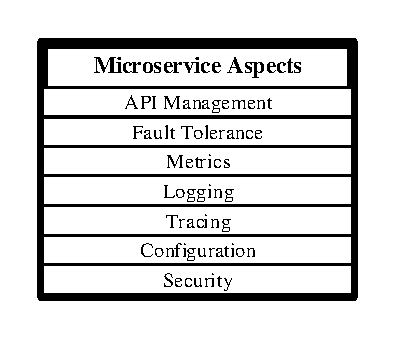
\includegraphics[scale=1]{images/esboc-requirement-services.pdf}
	\caption{Microservice aspects}
	\label{fig:esboc-aspects}
\end{figure} 

\subsection{Security}
\label{sec:esboc-aspects-security}
Distributed services need to be secured properly from unauthorized access, therefore the microservices will be secured with OAuth2. OAuth2 is a token based authentication scheme, which has become popular over past few years. There are several open source implementations for interacting with an authentication service via the OAuth2 scheme. The Integration Service must authenticate its client, the Application Service, against a central authentication service, whereby the Application Service will retrieve the access tokens from the central authentication service, and the Integration Service validates the provided token against the central authentication service\cite{OAuth2018}.

\subsection{Configuration}
\label{sec:esboc-aspects-config}
The Eclipse MicroProfile specifications provide the MicroProfile-Config specification, which provides an API to inject configuration parameters into CDI Beans. The injected configuration parameters are loaded from so called configuration sources. A configuration source can either be Java system properties, environment variables, properties files, YAML files, or custom implementations, for instance to retrieve configurations from a database. The services must be implemented in a way, to be configurable for different stages such as DEV (development) and PROD (production), whereby  the services are only allowed to use configuration parameters via injection\cite{EclipseMicroprofileConfig2018}.

\subsection{Tracing}
\label{sec:esboc-aspects-tracing}
The Eclipse MicroProfile specifications provide the MicroProfile-OpenTracing specification, which provides an API for tracing an application on a method level and across service boundaries. Distributed tracing allows to comprehend service or method call chains of distributed services. There is open source tooling available to analyze the collected tracing data, provided by the distributed services. The services must collect reasonable tracing information and send this data to a central tracing service\cite{CNCFOpentracing2018}.

\subsection{Logging}
\label{sec:esboc-aspects-logging}
Distributed logging allows to comprehend logs across service boundaries within a service call chain, whereby the logs of all involved services have to be marked with the same transaction id. There is open source tooling available to analyze the collected logs, provided by the distributed services. The services must provide all of their logging to a central service, whereby the logs must be marked with a transaction id, which is provided by the MicroProfile-OpenTracing-API. Optionally, the services are allowed to add additional markers, which can help developers and operators to analyze problems or to group service logs.

\subsection{Metrics}
\label{sec:esboc-aspects-metrics}
The Eclipse MicroProfile specifications provide the MicroProfile-Metric specification, which provides an API to define and manage metrics. Metrics allow to comprehend the state of a microservice, such as resource consumption, API calls, or failure counts. Metrics along with distributed tracing and distributed logging, provide the necessary data, developers and operators need to analyze failures in services, which occurred in service call chains. The services must collect reasonable metrics and publish those metrics, which can be made available to a central metric service\cite{EclipseMicroprofileMetrics2018}.

\subsection{Fault Tolerance}
\label{sec:esboc-requirements-service-fault}
The Eclipse MicroProfile specifications provide the MicroProfile-FaultTolerance specification, which provides an API to define fault tolerance behavior such as retries, timeouts, and error fall-backs. The fault tolerance of a service means, that if a depending service is not accessible at the time, a service must not fail immediately after the first try, but the service should retry to call the depending service for several times, and fail when all retries have failed. Such a behavior ensures, that short timed communication errors, redeployments, or overloads do not immediately cause a service to fail. The services must provide proper fault tolerance configuration and fall-back behavior, to be able to recover from such errors in a proper manner\cite{EclipseMicroprofileFault2018}.   

\subsection{API Management}
\label{sec:esboc-requirements-service-api}
The API management of a public API such as REST API and REST Models ensure, that the clients, using the public API, are not broken by changes, made on that API. There are several opinions on how API management can be done. A public API has to be stable per design, and needs to evolve and provide backward compatibility in a way, so that clients have enough time to catch up with the changes. Swagger has become very popular for documenting an API, whereby the documentation can be used to generate clients, provide documentation for developers and to test the public API. The services must be capable of migrating their public API in a way, that the clients are not broken by made changes. The services must provide a Swagger Documentation, and provide a capability to access the Swagger Documentation\cite{SmartBearSwagger2018, RestVersion2018}.

\section{Openshift Architecture}
\label{sec:esboc-design-oc}
Figure \vref{fig:esboc-design-openshift-project} illustrates the design of the Openshift Project, which will act as the ESB. As discussed in Section \vref{sec:paas-openshift-project}, Openshift isolates Kubernetes Namespaces  by bringing in the concept of an Openshift Project. Services in an Openshift Project, which are not exposed via an Openshift Route, are implicitly protected from access from external networks and other Openshift Projects. The Openshift Project will contain the Application Service, the Database Service and the Integration Service. The Application Service has access to the Internet, and will be accessed by the Client from the Internet via its public address. The Integration Service and the Database Service are not exposed to the Internet, and can only be accessed within the Openshift Project by their service names.

\begin{figure}[htbp]
	\centering
	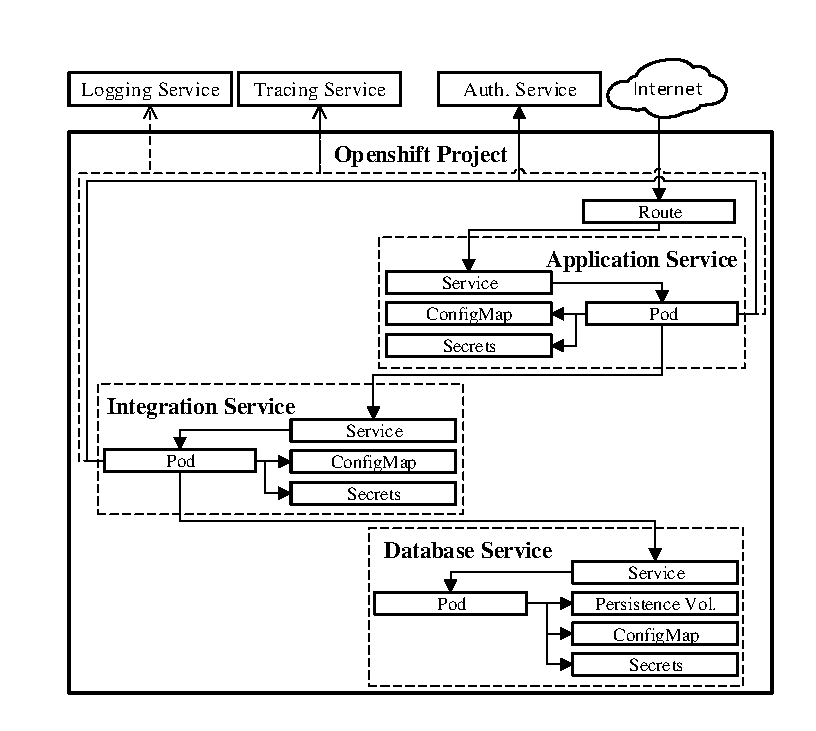
\includegraphics[scale=1]{images/esboc-design-openshift.pdf}
	\caption{Openshift Project architecture}
	\label{fig:esboc-design-openshift-project}
\end{figure} 

All services provide their tracing and logging data to external services, whereby no special configuration will be needed in Openshift, because Openshift allows services to access external networks. The mediation of the services is managed by Kubernetes Services, whereby the services communicate with each other via their service names, which ensures, that the communication stays within the Openshift Project. The Openshift Project must manage all configurations and secrets, which can be referenced by the services.

\section{Openshift Requirements}
\label{sec:esboc-requirements-oc}
The implementation of the Openshift Project such as templates and scripts, must be implemented under consideration of the principles of IaC, which have been discussed in Section \vref{sec:iac-principles}. Sticking to the principles of IaC will ensure, that the Openshift Project can effortlessly be managed and reproduced on any Openshift Cluster. \\

The Openshift Project will host the services and manage their configurations and secrets via Openshift ConfigMaps and Openshift Secrets, which have been discussed in Section \vref{sec:caas-kubernetes-objects}. The configurations and secrets are managed outside the service code bases, and are provided by the Openshift Project for a specific stage, the Openshift Project represents. The configurations and secrets are supposed to be managed by operators, and are only made available to the services during runtime, and shouldn't be accessible by developers. \\

The services must manage their integration into Openshift, by providing the necessary templates, whereby configurations and secrets are referenced by their predefined names. The services must expose all necessary configuration parameters, which allow to configure the service for a specific stage, whereby the Openshift Project will provide the proper configuration and secret values for the specific stage. \\

The implemented prototype will consist of two Openshift Projects, whereby one Openshift Project will host the tracing service, log aggregation service and authentication service, and the second Openshift project will host the ESB services along with the simulated external database, which will be integrated. \\

The following chapter will discuss the implementation of the designed prototype. 

%\chapter{Implementation ESB in Openshift}
\label{cha:esbi}
This chapter will discuss the implemented prototype, which has been designed in Chapter \vref{cha:esboc}. The implemented prototype uses lots of Java Enterprise Frameworks and Java Enterprise-Platform specifications, which are beyond the scope of this thesis, therefore a focus will be set on the implementations of the aspects discussed in Section \vref{sec:esboc-aspects}. Is is assumed, that the reader is familiar with Java Enterprise Development, Java Enterprise Frameworks, Maven and the microservices architecture. The implemented prototype is available on Github \footnote{https://github.com/cchet-thesis-msc/prototype}. The repository contains a \mentionedtext{README.adoc} file, which describes how to setup the prototype on a Windows Host. \\

The services are implemented as microservices, with their own life-cycle, and run as standalone applications in Docker Containers on the Openshift Cluster. The services communicate via REST with each other, whereby each service provides a proper managed public API and documentation. The code bases of the services are managed separately, which completely decouples the services from each other. \\

As the prototype illustrates, the ESB is represented by an Openshift Project on an Openshift Cluster, whereby the Openshift Cluster acts as the platform for the hosted services. The services will be hosted in an Openshift Project, whereby the Openshift Project provides features as discussed in Section \vref{sec:paas-openshift-project} for managing the life-cycle of the hosted services. The implemented resources for managing the Openshift Project are discussed in Section \vref{sec:esbi-openshift}. \\

The following Section will briefly introduce the technologies and frameworks, which were used for implementing the services, which are running on the Openshift Cluster.

\section{Microservice Technologies}
\label{sec:esbi-technolody-fis}
The following sections will give a brief introduction about the most important technologies and frameworks, used to implement the services as microservices. Each implemented service is setup the same way, because the concrete purpose of the service doesn't matter, when the microservices have to be integrated into a distributed service network. All of the following technologies and frameworks provide all necessary API, implementations, and tooling, for implementing a microservice with the Java Enterprise-Platform, which is hosted on an Openshift Cluster.

\subsection{JBoss Fuse Integration Services 2.0}
\label{sec:esbi-technology-fis}
JBoss Fuse Integration Services 2.0 is a set of tooling for developing services running on an Openshift Cluster. It provides Openshift integrations for different frameworks such as Spring Boot, Karaf or Camel. The services are started via an Java Agent such as Prometheus or Jolokia, which are used to monitor the services during runtime. Additionally, a Maven Plugin is provided, which allows to interact with the Openshift Cluster during a Maven build, whereby the service life-cycle on an Openshift Cluster can be managed via Maven Goals. JBoss Fuse Integration Services 2.0 allows developers to interact with an Openshift Cluster in a way like developers did before with an application server like Wildfly\cite{Prometheus2018, Jolokia2018}.

\subsection{Thorntail.io}
\label{sec:esbi-technology-swarm}
Thorntail.io, previously called Wildfly Swarm, is the Java Enterprise answer to Spring Boot, and is a framework based on Wildfly, which allows to package an application into an Uber-JAR. An Uber-JAR is a packaged standalone application, which can be started with the command \inlineJava{java -jar}. During the packaging, only those components of Wildfly are packaged, which are referenced and needed by the application. The application can then be started via \inlineBash{java -jar app.jar}, whereby the application server is bootstrapped programmatically. The Uber-Jar is a repackaged Java Web-Archive, which could be hosted on any Java application platform, which provides all of the referenced dependencies, which are added during the repackaging\cite{WildflySwarm2018,Wildfly2017}.  \\

During the implementation of the prototype, Wildfly Swarm has been renamed to Thorntail.io, whereby the Maven Group-Id has been renamed from \mentionedtext{org.wildfly.swarm} to \mentionedtext{io.thorntail}. The Maven Dependencies are still the same, but with a different Maven Group-Id.

\subsection{Fabric8}
\label{sec:esbi-technology-f8}
Fabric8 is an integrated development platform for developing applications on Kubernetes. Fabric8 provides a  Maven Plugin for the JBoss Fuse Integration Services 2.0, and focuses on building Docker Images, managing Kubernetes or Openshift resources, and deploying Java applications on Kubernetes or Openshift clusters. With the Maven Plugin, the interaction of developers with Openshift is reduced to a minimum, for instance, no custom Openshift BuildConfig has to be provided, because it is generated by the Maven Plugin itself\cite{Fabric82018}. \\

The following sections will discuss the implementations of the microservice aspects as discussed in Section \vref{sec:esboc-aspects}.

\section{Security}
\label{sec:esbi-security}
The services are secured with OAuth2, and authenticate their clients via Keycloak. Keycloak is used as the authentication service, and is a very popular open source identity and authentication application. Thorntail.io provides an integration into Keycloak via the Keycloak Adapter, which needs to be added as a dependency to the Maven \mentionedtext{pom.xml}. The adapter needs a configuration, to know what resources are secured.

\subsection{Service}
\label{sec:esbi-security-service}
This section will discuss the implementation of the security in the service implementations. Listing \vref{ls:esboi-security-pom} shows the dependency, which brings in the Keycloak Adapter. The Keycloak Adapter integrates itself into the Java Web-Security mechanisms, and can therefore be configured with Java Web-Security security constraints.

\begin{listing}[h]
	\xmlFile{\sourceDir/maven-keycloak-swarm.xml}
	\caption{Keycloak Adapter dependency in pom.xml}
	\label{ls:esboi-security-pom}
\end{listing}

Listing \vref{ls:esboi-security-yaml} shows an excerpt of the Thorntail.io configuration file \mentionedtext{project-stages.yml}, which configures the security constraints for the REST Endpoints.

\begin{listing}[h]
	\yamlFile{\sourceDir/project-stages-security.yml}
	\caption{Security configuration in project-stages.yml}
	\label{ls:esboi-security-yaml}
\end{listing}

The following two listings are excerpts of the \mentionedtext{deployment.yml} Openshift Template, which is managed in the service code base. Listing \vref{ls:esboi-security-oc-deployment-volume-secret} shows the specification of the secret injection into a Docker Volume. The secrets are injected as files, whereby the file name represents the secret key and the file content represents the secret value. Therefore, that the secrets are managed externally, the developers need to provide the secret name for the service deployment configuration. In this case an expression is used, which references a Maven Property, whereby the Maven Property can be provided in the \mentionedtext{pom.xml} or provided/overwritten by Java Options during the Maven Build.
\newpage

\begin{listing}[h]
	\yamlFile{\sourceDir/deployment-volume-secret.yml}
	\caption{Secret injection configuration in deployment.yml}
	\label{ls:esboi-security-oc-deployment-volume-secret}
\end{listing}

Listing \vref{ls:esboi-security-oc-deployment-volume-mount} shows the specification of the mount of the Docker Volume, which provides the secrets for the application. The mount path is also represented by a Maven Property, because this path is also used in the \mentionedtext{project-stages.yml} file, where it points to the service configuration source for the production stage. The secrets consumed by the services are used the same way as non-sensitive configurations, which are discussed in Section \vref{sec:esbi-configuration}.

\begin{listing}[h]
	\yamlFile{\sourceDir/deployment-volume-secret-container.yml}
	\caption{Secret volume mount configuration in deployment.yml}
	\label{ls:esboi-security-oc-deployment-volume-mount}
\end{listing}

\subsection{Openshift}
\label{sec:esbi-security-openshift}
This section will discuss the Openshift implementation, whereby the implementation is represented by a shell script, which manages the Openshift Secrets. The secrets are managed outside the code bases of the services, and are supposed to be maintained by operators.

\begin{listing}[h]
	\bashFile{\sourceDir/bash-oc-secret.txt}
	\caption{Openshift CLI commands for creating secrets}
	\label{ls:esboi-security-oc-secret}
\end{listing}
	
Listing \vref{ls:esboi-security-oc-secret} shows the Openshift CLI-Commands, which are used to create the Openshift Secrets. The first command creates an Openshift Secret from literal values, which provides the configurations for the service. The second command creates an Openshift Secret from a file, whereby the filename is the secret key and the file content is the secret value. 
\newpage

This section discussed the implementations, which are necessary to secure services hosted on an Openshift Cluster via OAuth2 with Keycloak. No source code is necessary, only configuration. The following section will discuss the configuration of the services, which can be applied to the security as well, because secrets in Openshift are used in the service implementations, the same way as configuration parameters.

\section{Configuration}
\label{sec:esbi-configuration}
The services use the MicroProfile-Config specification, to be configurable for multiple stages. The services consume the configuration parameters via injection, which can be provided from different configuration sources. Developers are bound to the configuration/secret name, keys, and value type. Developers are not bound to the configuration/secret source, which allows to provide configurations/secrets from different sources, and for different stages. 

\subsection{Service}
\label{sec:esbi-config-service}
This section will discuss the implementation of the configuration definition and usage. Listing \vref{ls:esboi-config-pom} shows the dependency, which brings in the MicroProfile-Config specification and implementation to enable injectable configurations.
 
\begin{listing}[h]
	\xmlFile{\sourceDir/maven-microprofile-config.xml}
	\caption{MicroProfile-Config dependency in pom.xml}
	\label{ls:esboi-config-pom}
\end{listing}

Listing \vref{ls:esboi-config-project-stages-dev} shows the definition of the configuration source in the \mentionedtext{project-stages.yml} for the development stage, whereby the configuration parameter values are provided hard coded.

\begin{listing}[h]
	\bashFile{\sourceDir/project-stages-micro-config-dev.yml}
	\caption{Hard coded configuration for development stage}
	\label{ls:esboi-config-project-stages-dev}
\end{listing}
\ \newpage

Listing \vref{ls:esboi-config-project-stages-prod} shows the definition of the configuration source in the \mentionedtext{project-stages.yml} for the production stage, whereby the configuration parameter values are loaded from files located in the configured directory. The directory location is represented by an expression referencing a Maven Property, because its used in multiple configuration files. The expression will be resolved as discussed in Section \vref{sec:esbi-security-service}.

\begin{listing}[h]
	\yamlFile{\sourceDir/project-stages-micro-config-prod.yml}
	\caption{External configuration for production stage}
	\label{ls:esboi-config-project-stages-prod}
\end{listing}

Listing \vref{ls:esboi-config-inject} shows the injection of the Keycloak Secrets into a CDI Bean, whereby the source of the configurations is not shown. The injected configuration properties are retrieved from an Openshift Secret, but are used in the source code the same way as configurations.

\begin{listing}[h]
	\javaFile{\sourceDir/java-config-inject.java}
	\caption{Injection of Keycloak configuration parameters}
	\label{ls:esboi-config-inject}
\end{listing}

\subsection{Openshift}
\label{sec:esbi-config-openshift}
The Openshift implementation has already been covered by Section \vref{sec:esbi-security-openshift}, because all of the configurations are managed as Openshift Secrets, because they contain sensitive data. 

\section{Tracing}
\label{sec:esbi-tracing}
The services use the MicroProfile-OpenTracing specification to provide tracing data to a central tracing service. Jaeger is used as the tracing service, which collects all tracing data and provides a GUI for analyzing the collected traces\cite{CNCFJaeger2018}. 

\subsection{Service}
\label{sec:esbi-tracing-service}
This section will discuss the implementation of the service tracing. Listing \vref{ls:esboi-tracing-pom} shows the dependency, which brings in the MicroProfile-OpenTracing specification and implementation to enable tracing. 

\begin{listing}[h]
	\xmlFile{\sourceDir/maven-microprofile-opentracing.xml}
	\caption{MicroProfile-OpenTracing dependency in pom.xml}
	\label{ls:esboi-tracing-pom}
\end{listing}

Listing \vref{ls:esboi-tracing-project-stages} shows the configuration  in the \mentionedtext{project-stages.yml}, for the integration into the Jaeger tracing service, whereby the configuration parameters are provided by Maven Properties, environment variables and literals. The System Property JAEGER\_ENDPOINT defines the HTTP collector endpoint of the Jaeger tracing service, and is provided via an environment variable, which gets injected from an Openshift ConfigMap.

\begin{listing}[h]
	\yamlFile{\sourceDir/project-stages-opentracing.yml}
	\caption{Configuration of Jaeger integration in project-stages.yml}
	\label{ls:esboi-tracing-project-stages}
\end{listing}

Listing \vref{ls:esboi-tracing-java} shows a class which is annotated with \inlineJava{@Traced} on class level, which enables tracing for all methods within this class. The annotation \inlineJava{@Traced} enables a CDI Interceptor, which implements the tracing logic. \\

\begin{listing}[h]
	\javaFile{\sourceDir/java-tracing.java}
	\caption{Traced CDI Bean}
	\label{ls:esboi-tracing-java}
\end{listing}
\ \newpage

A trace is a set of so called spans, whereby a span represents one call in a call chain and contains meta-data of the call, such as the call duration. The CDI Interceptor creates a new span for each method invocation, and appends the created span to an existing parent span, or the created span is the parent span. 

\subsection{Openshift}
\label{sec:esbi-tracing-openshift}
The communication between the services and the tracing service is performed via HTTP, therefore Openshift does need any special configuration. Openshift doesn't interfere with outgoing connections, only incoming.

\section{Logging}
\label{sec:esbi-logging}
The services provide logging to a central log aggregation service. Graylog is used as the log aggregation service, which collects all logging data and provides a GUI for analyzing the aggregated logs\cite{Graylog2018}.

\subsection{Service}
\label{sec:esbi-logging-service}
This section will discuss the implementation of the service logging. Listing \vref{ls:esboi-logging-pom} shows the dependency, which brings in the Thorntail.io logging implementation, which needs to be configured to know how and where to send the produced logs.

\begin{listing}[h]
	\xmlFile{\sourceDir/maven-swarm-logging.xml}
	\caption{Logging dependency in pom.xml}
	\label{ls:esboi-logging-pom}
\end{listing}

The provided logging implementation of Thorntail.io does not support the used Graylog service, therefore the library logstash-gelf was added, which supports Graylog and provides a Wildfly compatible log handler, which can be used with Thorntail.io. The library is integrated via a custom JBoss Module, because it is only needed during runtime. The module.xml for the JBoss Module for logstash-gelf was defined at src/main/resources/modules/<module\_name>/main/module.xml. Listing \vref{ls:esboi-logging-logstash} shows the custom JBoss Module \mentionedtext{module.xml}, which integrates the logstash-gelf library. The defined artifacts are downloaded by Thorntail.io during the re-packaging phase of the Maven Build\cite{LogstashGelf2018}.
\newpage

\begin{listing}[h]
	\xmlFile{\sourceDir/paluch-module.xml}
	\caption{JBoss module.xml for integrating logstash-gelf}
	\label{ls:esboi-logging-logstash}
\end{listing}

The following listings are part of the \mentionedtext{project-stages.yml}, and configure the logging for the different stages. Listing \vref{ls:esboi-logging-format-project-stages} shows the configuration of the logging format, which uses Mapped-Diagnostic-Context (MDC) parameters to mark a log entry with the transaction id, provided by the tracing implementation. The configured formatter is defined globally, therefore it will used for all stages.

\begin{listing}[h]
	\yamlFile{\sourceDir/project-stages-logging-format.yml}
	\caption{Logging format configuration in project-stages.yml}
	\label{ls:esboi-logging-format-project-stages}
\end{listing}

Listing \vref{ls:esboi-logging-dev-project-stages} shows the logging configuration for the development stage.

\begin{listing}[h]
	\yamlFile{\sourceDir/project-stages-logging-dev.yml}
	\caption{Logging configuration for development stage in project-stages.yml}
	\label{ls:esboi-logging-dev-project-stages}
\end{listing}

Listing \vref{ls:esboi-logging-prod-project-stages} shows the configuration in the \mentionedtext{project-stages.yml} for the logging of the production stage, whereby logs are send to a central log aggregation service. A log handler of the logstash-gelf library is configured, which sends the logs to the log aggregation service via HTTP.

\begin{listing}[h]
	\yamlFile{\sourceDir/project-stages-logging-prod.yml}
	\caption{Logging configuration for production stage in project-stages.yml}
	\label{ls:esboi-logging-prod-project-stages}
\end{listing}

Listing \vref{ls:esboi-logging-java-transaction-id} shows the implementation of the interface \mentionedtext{ContainerRequestFilter} provided by the JAX-RS specification, which is used to capture the current trace transaction id on the REST Endpoints. The implementation is depending on the Uber MicroProfile-OpenTracing implementation, because the specification itself doesn't provide an accessor for the transaction id yet. The captured transaction id is set into MDC, whereby the formatter, defined in Listing \vref{ls:esboi-logging-format-project-stages}, references the MDC parameter. In the production stage, the configured log handler sends the MDC parameters to the log aggregation back-end as own fields.

\begin{listing}[h]
	\javaFile{\sourceDir/java-logging-tracing-id.java}
	\caption{Capture of the tracing id via a JAX-RS Filter}
	\label{ls:esboi-logging-java-transaction-id}
\end{listing} 

Listing \vref{ls:esboi-logging-java-producer} shows the CDI Producer method, which provides the logger instances for injection points. The logger is produced for the Dependent Scope, which means, that the life-cycle of the logger instance is managed by the CDI Bean, which gets the logger injected.

\begin{listing}[h]
	\javaFile{\sourceDir/java-logging-producer.java}
	\caption{CDI Producer for dependent scoped logger instances}
	\label{ls:esboi-logging-java-producer}
\end{listing} 

Listing \vref{ls:esboi-logging-java} shows a class using an injected logger to log a info message. As this examples illustrates, the user code has no knowledge about a log aggregation back-end or about a transaction id.

\begin{listing}[h]
	\javaFile{\sourceDir/java-logging.java}
	\caption{Logger usage in a CDI Bean}
	\label{ls:esboi-logging-java}
\end{listing} 

\subsection{Openshift}
\label{sec:esbi-logging-openshift}
The services send their logs to a central log aggregation service via HTTP, and therefore no special settings for Openshift necessary. Nevertheless, logs send to the console are collected by Openshift and can be analyzed in the Openshift Web-Console as well.

\section{Fault Tolerance}
\label{sec:esbi-fault}
The services use the MicroProfile-FaultTolerance specification to define fault tolerance behavior on methods. Hystrix is a popular framework for failure handling in applications, was the inspiration for the MicroProfile-FaultTolerance specification, and is used as the back-end for the Thorntail.io provided dependency\cite{NetflixHystrix2018}.

\subsection{Service}
\label{sec:esbi-fault-service}
This section will discuss the implementation of the service fault tolerance. The services use the MicroProfile-FaultTolerance specification to define the service fault tolerance behavior, which defines the service resilience. Listing \vref{ls:esboi-fault-tolerance-pom} shows the dependency, which brings in the fault tolerance specification and implementation.

\begin{listing}[h]
	\xmlFile{\sourceDir/maven-microprofile-fault-tolerance.xml}
	\caption{MicroProfile-FaultTolerance dependency in pom.xml}
	\label{ls:esboi-fault-tolerance-pom}
\end{listing}

Listing \vref{ls:esboi-fault-tolerance-java} shows the CDI Producer method for producing the Oauth token, whereby the method defines fault tolerance behavior via annotations. The applied annotations active CDI Interceptors, which implemented the specific fault tolerance logic. The special use of the method as a CDI Producer doesn't affect the fault tolerance logic. Each time when the producer method is called a token request is send to Keycloak to retrieve an access token. The invocation is retried 5 times with a 100 millisecond delay, and each invocation is timed out after 5 seconds.

\begin{listing}[h]
	\javaFile{\sourceDir/java-fault-tolerance.java}
	\caption{Fault tolerance definition on a CDI Producer method}
	\label{ls:esboi-fault-tolerance-java}
\end{listing} 

\subsection{Openshift}
\label{sec:esbi-fault-openshift}
The fault tolerance behavior as discussed in Section \vref{sec:esbi-fault-service} only affects the service itself and not Openshift. But, Openshift provides a kind of fault tolerance, for instance by restarting crashed Pods.

\section{API-Management}
\label{sec:esbi-api}
The services use Swagger to provide documentation for their REST API. Swagger provides an intermediate format, which can be used by tooling for testing and client generation. The REST API represents the public view of the service, which is implemented in a way, so that it is decoupled from the service logic, and supports several ways to perform API migrations. \\

The following sections will discuss the implementation of the REST API-Management on the service side, and the REST API usage on the client side. Both use Swagger, whereby the service provides Swagger Documentation, and the clients are generated by using the service provided Swagger Documentation.

\subsection{Service}
\label{sec:esbi-api-service}
This section will discuss the management and implementation of the service REST API. Listing \vref{ls:esboi-api-service-pom} shows the dependencies, which bring in the 
\begin{itemize}
	\item the Java BeanValidation implementation, 
	\item the JAX-RS Server implementation,
	\item the JAX-RS Server Java-BeanValidation integration,
	\item and the Swagger specification and implementation. 
\end{itemize}

\begin{listing}[h]
	\xmlFile{\sourceDir/maven-swagger-service.xml}
	\caption{JAX-RS/BeanValidation/Swagger dependencies in pom.xml}
	\label{ls:esboi-api-service-pom}
\end{listing}

Listing \vref{ls:esboi-api-swagger-conf} shows an excerpt of the  \mentionedtext{project-stages.yml}, which configures Swagger for the documented service. During startup, Swagger will scan the configured packages for interfaces and classes, which provide documentation in form of Swagger Annotations. The scanned documentations are written to a file named \mentionedtext{swagger.json}, which contains the Swagger Documentation of the service REST API.  
\newpage  

\begin{listing}[h]
	\yamlFile{\sourceDir/project-stages-swagger.yml}
	\caption{Swagger configuration in project-stages.yml}
	\label{ls:esboi-api-swagger-conf}
\end{listing}

Listing \vref{ls:esboi-api-swagger-java} shows an interface, which specifies a REST Endpoint via JAX-RS Annotations, and provides documentation via Swagger Annotations. Additionally, Java BeanValidation-Annotations are used to define constraints for the input arguments of the REST Operations, so that validation is applied on all incoming requests. The JAX-RS, Java BeanValidation, and Swagger Annotations, are scanned and applied to the generated Swagger Documentation.

\begin{listing}[h]
	\javaFile{\sourceDir/java-swagger.java}
	\caption{JAX-RS interface with Swagger Annotations}
	\label{ls:esboi-api-swagger-java}
\end{listing}

\subsection{Client}
\label{sec:esbi-api-client}
This section will discuss the implementation of the REST Client, which is generated by the Swagger Maven-Plugin by using the service provided \mentionedtext{swagger.json} file. The following listings show the configuration of the Maven Plugins, which are used to generate a REST Client from a Swagger Documentation during a Maven Build. \\

Listing \vref{ls:esboi-api-client-add-sources-pom} shows the configuration of the Maven Helper-Plugin in the consumer service \mentionedtext{pom.xml}, which is used to add the generated REST Client sources for the compilation. The source directory points to the directory, where the generated REST Client sources are located.
\newpage

\begin{listing}[h]
	\xmlFile{\sourceDir/maven-swagger-client-add-sources.xml}
	\caption{Maven Helper-Plugin configuration in pom.xml}
	\label{ls:esboi-api-client-add-sources-pom}
\end{listing}

Listing \vref{ls:esboi-api-client-clean-pom} shows the configuration of the Maven Clean-Plugin in the consumer service \mentionedtext{pom.xml}, which is used to clean the unwanted generated sources and resources. The Swagger Maven-Plugin generates a standalone REST Client, which cannot be turned off, but only the plain generated models and interfaces are needed. 

\begin{listing}[h]
	\xmlFile{\sourceDir/maven-swagger-client-clean.xml}
	\caption{Maven Clean-Plugin configuration in pom.xml}
	\label{ls:esboi-api-client-clean-pom}
\end{listing}

Listing \vref{ls:esboi-api-client-swagger-plugin-pom} shows the Swagger Maven-Plugin configuration in the consumer service \mentionedtext{pom.xml}, which is used to generate the REST Client during the Maven Build. Custom Swagger Code-Generator templates are used, due to the fact that, there is no Swagger Code-Generator, which only generates plain JAX-RS interfaces and models. 
\newpage

\begin{listing}[h]
	\xmlFile{\sourceDir/maven-swagger-client-swagger-plugin.xml}
	\caption{Swagger Maven-Plugin configuration in pom.xml}
	\label{ls:esboi-api-client-swagger-plugin-pom}
\end{listing}

Listing \vref{ls:esboi-api-client-api-java} shows an excerpt of a generated JAX-RS interface, which was generated from a Swagger Documentation, which was provided by a generated \mentionedtext{swagger.json} file. The generated JAX-RS interface is very similar to the original JAX-RS interface, but could contain differences, for instance when a REST Operation parameter of type string was documented as value type number.

\begin{listing}[h]
	\javaFile{\sourceDir/java-swagger-client.java}
	\caption{Generated JAX-RS interface}
	\label{ls:esboi-api-client-api-java}
\end{listing}

Listing \vref{ls:esboi-api-client-api-builder-java} shows how to build an REST-Client for the generated JAX-RS interfaces, whereby developers work with the generated API, and the logic for handling the request and response is provided by RESTEasy. Changes made to the Swagger Documentation could cause compile errors, because the signature of the generated interface could differ from the previous generated version. Therefore, the usage of the REST Client is type safe. The MicroProfile-OpenTracing implementation provides a JAX-RS Client-Filter, which ensures, that the REST Clients contribute to the tracing. A custom JAX-RS Client-Filter has been implemented, which retrieves the OAuth2 Token from the CDI Container, and sets the token on the HTTP Authentication-Header of the client request\cite{RESTEasy2018}.

\begin{listing}[h]
	\javaFile{\sourceDir/java-swagger-client-builder.java}
	\caption{Building a type safe REST client}
	\label{ls:esboi-api-client-api-builder-java}
\end{listing}

In the prototype, the built REST Clients are injectable into CDI Beans, whereby the Rest Clients are managed by a custom proxy, which applies proper fault tolerance behavior to the REST Client method calls.

\subsection{Openshift}
\label{sec:esbi-api-openshift}
The REST API-Management and migration doesn't affect Openshift, because the services REST API is either accessible only within the Openshift Project network, or is exposed via a single Openshift Route. Openshift doesn't provide any mechanisms for redirecting requests to other services based on path conditions, as for instance Nginx is capable to do so. 

\section{Openshift Project}
\label{sec:esbi-openshift}
This section will discuss the implementation of the Openshift Project, which represents the ESB. The implementations are represented by scripts, configurations and secrets, which ensure that the Openshift Project is properly setup, and provides all resources needed by the services, such as Openshift ConfigMaps and Openshift Secrets. The Openshift resources, which are consumed by the services, are managed by one script per service. The scripts, configurations and secrets are managed by operators, who ensure, that the Openshift Projects are properly setup, and provide all Openshift resources for the services, for a specific stage, an Openshift Project represents.
\newpage

The Openshift related resources of a service, such as the scripts, configurations and secrets, are organized in the following directory structure.
\begin{itemize}
	\item \textbf{/<service\_name>} is the directory holding all service related resources.
	\item \textbf{/<service\_name>/config/<stage>} is the directory holding the service configuration for a specific stage.
\end{itemize}

The stage is defined via the environment variable \mentionedtext{STAGE}, which acts as the selector for the configurations to use as shown in Listing \vref{ls:esboi-openshift-oc-service}.

\subsection{Scripts}
\label{sec:esbi-openshift-secrets}
This section will discuss the implemented scripts for managing a service and its needed Openshift resources in Openshift. Listing \vref{ls:esboi-openshift-oc-service} shows an excerpt of an implemented script for a service, which manages Openshift Secrets, and provides functions for scaling. The creation of secrets has already been discussed in Section \vref{sec:esbi-security-openshift}. The Openshift Secrets could also have been created from Openshift Templates, whereby the secrets are either hard-coded in the Openshift Templates, or are provided via Openshift Template-Parameters. The scaling of the service could also be performed via the Fabric8 Maven-Plugin, but operators usually don't have access to the service code base.

\begin{listing}[h]
	\bashFile{\sourceDir/bash-oc-service.sh}
	\caption{Shell script for managing a service via the CLI}
	\label{ls:esboi-openshift-oc-service}
\end{listing}

The following chapter will evaluate and analyze the implemented prototype, if the prototype fulfills the specifications of Chapter \vref{cha:esboc}, and if the prototype is a valid representation for an ESB in Openshift.



%\chapter{Discussion ESB in Openshift}
\label{cha:esbd}
This chapter will discuss the implemented prototype of Chapter \vref{cha:esbi}, and will discuss some important tasks such as 
\begin{itemize}
	\item managing multiple environments,
	\item managing service security,
	\item managing multiple service versions,
	\item managing public API migration,
	\item and managing Adapters and Message Translators as services,
\end{itemize}
which are very important, when running an ESB on Openshift. Whenever possible, Openshift will be compared to JBoss EAP, which can be used as the platform for the ESB middleware JBoss Fuse, as discussed in Section \vref{fig:esb-software-architecture}. \\

The prototype implementation represents an ESB running on Openshift, but is actually nothing more than an application represented by several microservices, running on a PaaS platform. Instead of managing a monolithic ESB application, as discussed in Section \vref{sec:esb-as-software}, the ESB application is split into independent microservices, which are managed completely separately. Because of the usage of Openshift as the platform, the implemented services of the prototype are distributed services per default, which is the nature of Kubernetes, which is the base for Openshift. Openshift takes care of the distribution of the Pods within the Openshift Cluster, and ensures, that the Pods are accessible via their related service abstraction. \\

When splitting any monolithic application into independent microservices, then the sum of resources needed by all microservices of the ESB, will be higher as the resources needed by a monolithic ESB. With microservices more resources are needed, due to the fact, that each microservice brings in its own runtime environment, whereby the monolithic ESB runs in one runtime environment. This a trade off, which needs to be considered when designing microservices for an ESB, or when splitting up a monolithic application to a microservice architecture. \\

Table \vref{tab:esbd-resource-monolith-vs-microservice} illustrates not a real world example, but shows the trend of the resource need of the whole application, when a monolithic application is split up into microservices. When the application is split up into too many microservices, then the needed resources increase drastically. The illustrated resources for the microservices are representing the minimum assigned resources the platform has to provide, to ensure, that all microservices will have the assigned resources available when they are under load.

{\renewcommand{\arraystretch}{1.2}%
\newcolumntype{m}{>{\hsize=.3\hsize}X}%
	\begin{table}[h]
		\begin{tabularx}{\textwidth}{ m|c|c|c|c }	
			\textbf{Resource}    & \textbf{Monolith} & \textbf{1 Micros.} & \textbf{10 Micros.} & \textbf{20 Micros.} \\  \hline
			\textit{$CPU/Cores$} & 2                 & 0.5                & 5                   & 10 \\
			\textit{$RAM/GB$}    & 3                 & 0.5                & 5                   & 10 \\ \hline
		\end{tabularx}
		\caption{Resource comparison of monolith and microservices}
		\label{tab:esbd-resource-monolith-vs-microservice}
\end{table}}

\section{Service mediation}
\label{sec:esbd-service-mediation}
The SOA Patterns specify a mediation layer as layer, which facilitates the communication across multiple services by providing an abstraction layer, which decouples the services from each other. The mediation layer ensures, that services can seamlessly communicate with replaced, relocated, or newly released services instances. Kubernetes provides the concept of a Kubernetes Service, which mediates the requests among multiple service instances represented by the service Pods. The Kubernetes Service is a content unaware mediator, because the message remains unchanged, and only mediation between service instances is supported.

\begin{figure}[htbp]
	\centering
	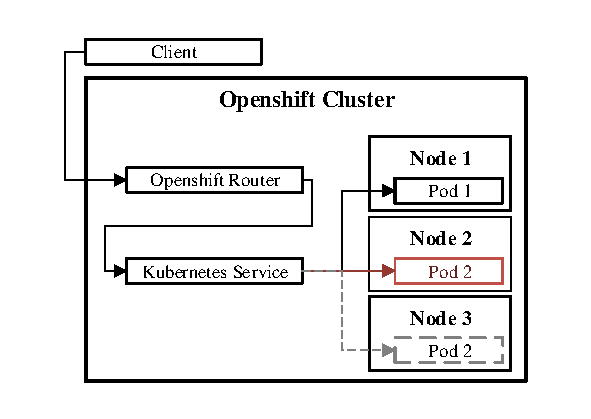
\includegraphics[scale=1]{images/esbd-service-mediation.pdf}
	\caption{Openshift Service mediation}
	\label{fig:esbd-service-mediation}
\end{figure}

Figure \vref{fig:esbd-service-mediation} illustrates a scenario, where the service Pod 2 on Node 2 fails, and gets recreated on Node 3, whereby it gets a new IP address assigned. The Kubernetes Service is aware, that Pod 2 has been recreated on Node 3, and will balance the requests to the recreated Pod 2 located on Node 3, when Pod 2 is fully up and running. A Kubernetes Service performs a simple mediation by abstracting service Pods via service names, and load balancing of the requests to the service Pods depending on the chosen algorithm. \\

With an ESB, there is no central mediator needed, because an ESB is a distributed architectural model, which has no central component like a Hub and Spoke architecture. If message translation is needed, because of a consumer incapability of supporting the ESB used message format and protocols, then an adapter and message translator is needed, as discussed in Section \vref{sec:esbd-adap-trans-service}. \\

The following sections will discuss the tasks introduced in the beginning of this chapter, and will show, that these task can be performed on the implemented prototype.

\section{Managing Multiple Environments}
\label{sec:esbd-multiple-env}
An ESB is commonly hosted on multiple environments, whereby at least one productive and one testing environment should be present. These environments were commonly a VM, which provided the runtime environment for the ESB middleware. As the prototype shows, the environment is now represented by an Openshift Project, which can be reproduced via scripts as discussed in Section \vref{sec:esbi-openshift}. \\

The services hosted on the ESB are using Fuse Integration Service 2.0 and its provided tooling, which ensure, that the services are properly encapsulated in a container, and are properly managed in Openshift. Therefore, the service developers provide the necessary Openshift Templates, which has the effect, that the operators have no interaction with the service artifacts and service runtime environments anymore. Operators have to manage
\begin{itemize}
	\item the Openshift Project, which contains the services,
	\item the Openshift ConfigMaps, which hold the service non-sensitive configuration,
	\item and the Openshift Secrets, which hold the sensitive service configuration.
\end{itemize} 
\ \\
Figure \vref{fig:esbd-multi-stage-env} illustrates the management and provisioning of multiple environments for an ESB, whereby the environment is represented by an Openshift Project. The Management Server pulls the scripts and Openshift Templates from a VCS Server, and the configurations from a Configuration Server, and uses them to provision new Openshift Projects, or manage existing ones. The scripts and Openshift Templates are separated from the configurations, which are providing the values for the scripts and Openshift Template-Parameters. With such an approach, the infrastructure becomes reproducible, versioned, and therefore consistent and disposable. These characteristics of IaC have been discussed in Chapter \vref{cha:iac}.
\newpage 

\begin{figure}
	\centering
	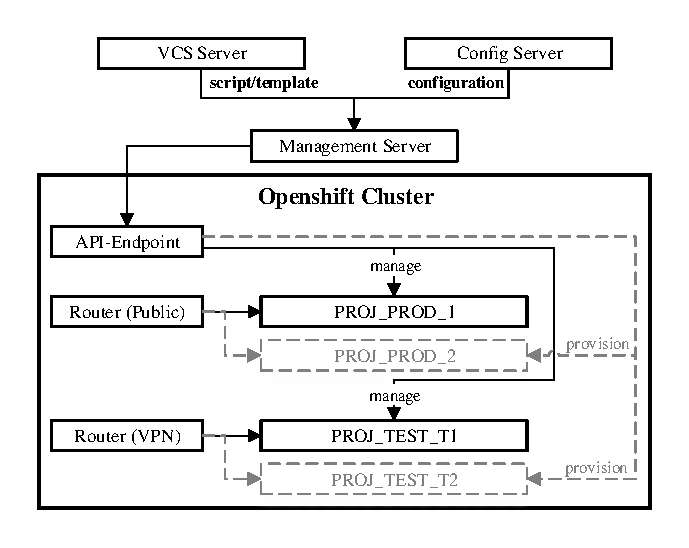
\includegraphics[scale=1]{images/esbd-multi-stage-env.pdf}
	\caption{Management and provisioning of multiple environments}
	\label{fig:esbd-multi-stage-env}
\end{figure}

The interaction of the Management Server, VCS Server and Configuration Server, as illustrated in Figure \vref{fig:esbd-multi-stage-env}, is similar to the Figure \vref{fig:reproduce-infrastructure}, which illustrated how a system can be reproduced with parametrized templates and an IaC tool. The Openshift CLI provides functionality to manage Openshift Objects, which is what needs to be done, when providing an environment in form of an Openshift Project.  \\

Table \vref{tab:esbd-multi-stage-env} compares the Openshift and JBoss EAP contained mechanisms, which provide the listed infrastructure features. As illustrated in the table, Openshift provides networking and isolation features, which are provided to JBoss EAP by its hosting environment such as a VM. Except of the networking and isolation feature, JBoss EAP supports all other features either natively or by supporting a third party library. Nevertheless, Openshift combines all features in one platform, and makes them manageable via Openshift Templates and the Openshift CLI. \\

Openshift runs Docker Containers, and therefore the programming language, the service was implemented with, doesn't matter, as long as the services can run in a container. Also, services hosted on PaaS platforms communicate via standard Protocols such as HTTP, which is commonly supported by almost any programming language. JBoss EAP on the contrary, runs only Java applications.
\newpage

{\renewcommand{\arraystretch}{1.2}%
\begin{table}[h]
	\begin{tabularx}{\textwidth}{ X|X|X }	
	  \textbf{Feature}                  & \textbf{Openshift}         & \textbf{JBoss EAP} \\  \hline
	  \textit{Staging}                  & Openshift Project          & Server Instance \\  \hline
	  \textit{Management}               & Openshift CLI              & JBoss CLI \\
	                                    & Openshift Web-Console      & JBoss Web-Console \\
	                                    & Openshift REST-API         & \\  \hline
	  \textit{Networking}               & Openshift Project          & None (external) \\
	                                    & Openshift Service          & \\  
	                                    & Openshift Route            & \\  
	                                    & Openshift Router           & \\  \hline
	  \textit{Isolation}                & Openshift Project          & None (external) \\  \hline
	  \textit{Configuration/Secrets}    & Openshift ConfigMaps       & Java System-Properties  \\
	                                    & Openshift Secrets          & Environment Variables \\
	                                                                && Password Vault \\  \hline
	  \textit{Service Distribution}     & Openshift Worker-Node      & Single JVM \\ 
			                                                        && Karaf \\  
			                                                        && OSGI \\  \hline
	  \textit{Service Roll-out}         & Recreate                   & Framework dependent, \\ 
			                            & Rolling                    & normally recreate \\ \hline
	  \textit{Language Support}         & All runnable in containers & Java \\
	\end{tabularx}
	\caption{Infrastructure feature comparison}
	\label{tab:esbd-multi-stage-env}
\end{table}}

The next section will discuss the service security within an Openshift Project, which can be managed the same way, as discussed in this section. Additionally to the security, provided by the isolation feature of an Openshift Project, the Management Server of Figure \vref{fig:esbd-multi-stage-env} could also manage custom security configurations, which can be managed via the Openshift CLI as well. 

\section{Managing Service Security}
\label{sec:esbd-service-security}
With a common ESB middleware, the services are protected by running within a single runtime environment, or by security features provided by a supported third party library. In an Openshift Project, the services are implicitly protected by being isolated in a Kubernetes Namespace, as discussed in Section \vref{sec:paas-openshift-project}, whereby the namespace of an Openshift Project cannot be accessed by other Openshift Projects without additional configuration. Services, which are supposed to be accessible from external networks, have to be explicitly exposed via an Openshift Route, which can handle secured connections, similar to an reverse proxy.
\newpage

\begin{figure}[htbp]
	\centering
	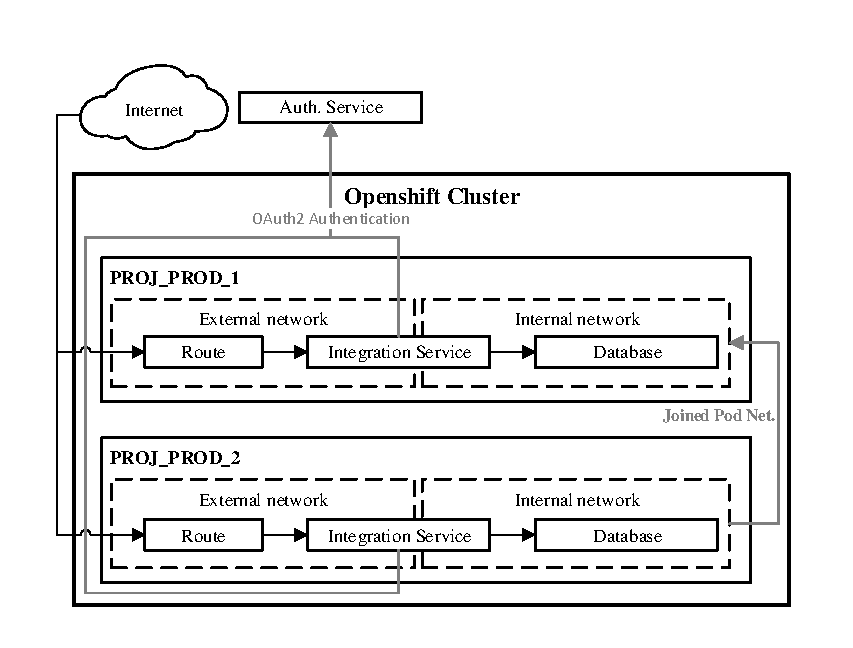
\includegraphics[scale=1]{images/esbd-service-security.pdf}
	\caption{Service security in an Openshift Project}
	\label{fig:esbd-service-security}
\end{figure}
\ \\
Figure \vref{fig:esbd-service-security} illustrates an example, similar to the implemented prototype, whereby two Openshift Projects host the same services, and where the Pod Networks of the two Openshift Projects are joined. The joined Pod Networks allow services hosted in project PROJ\_PROD\_2 to access services hosted in project PROJ\_PROD\_1 by their fully qualified service name. The fully qualified service name has the form of \mentionedtext{<service>.<project\_namespace>.svc.cluster.local}. Joining two Pod Networks is performed by Openshift Cluster administrators, and cannot be performed by developers. \\

Additionally to the isolation of the services within the Openshift Project, the Integration Service is secured via OAuth2, whereby the resource access is controlled by a central Authentication Server. On the one hand, the services are isolated within a Kubernetes Namespace, and on the other hand, additional security, such as access control, has to be provided by the service itself, because Openshift doesn't provide such a feature. It is not meant to isolate services from each other within an Openshift Project, because an Openshift Project, in particular a Kubernetes Namespace, should only contain a set of services, which don't have to be isolated from each other. \\
\newpage

Table \vref{tab:esbd-service-security} compares the Openshift and JBoss EAP contained mechanisms, which provide the listed security features. As illustrated in the table, Openshift doesn't provide any support for access control on the service level, which is normal for a PaaS platform, such as Openshift. The services, running in Docker Containers on an Openshift Cluster, have to implement access control, or have to use third party frameworks, such as the Keycloak Adapter, which provides access control features as discussed in Section \vref{sec:esbi-security}. JBoss EAP on the other hand is a Java Application-Platform, which provides support for access or user control for several providers. 

{\renewcommand{\arraystretch}{1.2}%
	\begin{table}[h]
		\begin{tabularx}{\textwidth}{ X|X|X }	
			\textbf{Feature}                 & \textbf{Openshift}      & \textbf{JBoss EAP} \\  \hline
			\textit{Network Isolation}       & Openshift Project       & None (VM) \\  \hline
			\textit{HTTPS}                   & Openshift Router        & Reverse Proxy \\
			                                 & Openshift Route         & Endpoint Configuration \\  \hline
            \textit{Access Control}          & None (external)         & Endpoint Configuration \\
                                                                      && Internal User-Database \\ 
                                                                      && External User-Database \\  \hline
            \textit{Single-Sign-On}          & None (external)         & Endpoint Configuration \\
                                                                      && Several SSO providers \\  \hline
		\end{tabularx}
		\caption{Security feature comparison}
		\label{tab:esbd-service-security}
\end{table}}

Openshift doesn't provide access control features to secure service resources, but provides security features such as user/group/role management, project permission management, Pod Network management, or quota management for Openshift Objects, such as Replication Controllers. Openshift uses Software Defined Networks (SDNs), whereby 
the services don't have to handle communication security, because the Openshift Cluster will take care of it. Exposed services are connected to an Openshift Route, whereby the Openshift Route, which acts as the reverse proxy, applies security to the communication on the external network. Within the isolated Pod Network, the services don't have to handle communication security, because this is handled by the Openshift Cluster. 

\section{Managing Multiple Service Versions}
\label{sec:esbd-multi-version-service}
Sometimes it is necessary to run multiple versions of a service, for instance, if a new version is released, or if a consumer is not capable of migrating to the new version, but provides a significant business value for the enterprise. Openshift provides mechanisms to run multiple versions of a service in several ways. Figure \vref{fig:esbd-service-multiple-versions} illustrates some scenarios for running multiple service versions on Openshift, whereby the illustrated scenarios of PROJ\_1 and PROJ\_2 are possible, because the old service version is N-1 compatible. N-1 compatibility means, that the service in the old version is capable of reading data written by the service in the new versions.
\newpage

\begin{figure}[htbp]
	\centering
	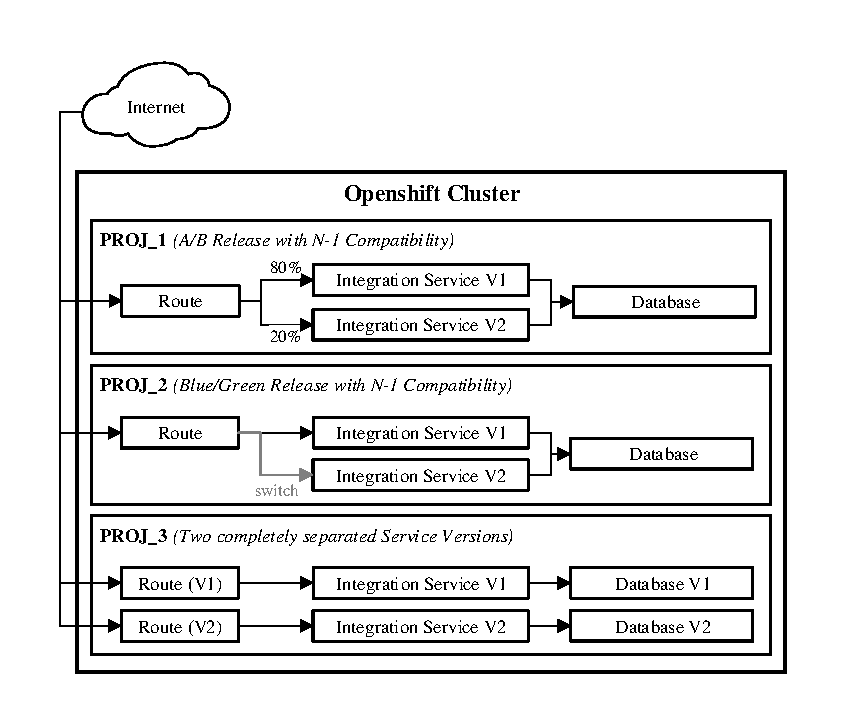
\includegraphics[scale=1]{images/esbd-service-multiple-versions.pdf}
	\caption{Running multiple service versions on Openshift}
	\label{fig:esbd-service-multiple-versions}
\end{figure}

\emph{PROJ\_1} of Figure \vref{fig:esbd-service-multiple-versions} illustrates an A/B Release, which is used to run the old and new version of a service in parallel, whereby a portion of the service consumers get access to the new version, while the rest of the service consumers are still using the old version. A/B Releases are used to validate the new version in the production environment, before fully releasing it to all consumers. In this scenario, the requests are load balanced by the Openshift Route to either the new or old service version. \\ 

\emph{PROJ\_2} of Figure \vref{fig:esbd-service-multiple-versions} illustrates a Blue/Green Release, which is used to run the old and the new version of a service in parallel, whereby the Openshift Route switches between the old and new service version. In this scenario, all service consumer access the same service version, which is currently accessible by the Openshift Route. \\

\emph{PROJ\_3} of Figure \vref{fig:esbd-service-multiple-versions} illustrates two service versions running completely separated in parallel, whereby both versions are accessible via their own Openshift Route. This scenario is not a release scenario, and should be used if multiple service versions have to be provided, for instance, if a customer cannot switch to the new version, but provides a significant business value to the enterprise. \\

Table \vref{tab:esbd-service-multiple-versions} compares the Openshift and JBoss EAP contained mechanisms, which provide the listed release features. Multiple service versions on an Openshift Cluster are represented by separate Openshift Service objects, whereby with JBoss EAP, multiple service versions are either represented by separate JBoss EAP instances, or deployment contexts on a single JBoss EAP instance. With JBoss EAP version switching and weighted routing can be performed by an external reverse proxy, which in Openshift can be performed by an Openshift Route.

{\renewcommand{\arraystretch}{1.2}%
 \newcolumntype{m}{>{\hsize=.32\hsize}X}%
	\begin{table}[h]
		\begin{tabularx}{\textwidth}{ X|X|X }	
			\textbf{Feature}                  & \textbf{Openshift}      & \textbf{JBoss EAP} \\  \hline
			\textit{Multiple Service Versions}& Openshift Service       & Multiple EAP instances \\
											  & Openshift Route    	    & Multiple deployment contexts \\ \hline
			\textit{Weighted Routing}         & Openshift Route         & None (external) \\  \hline
			\textit{Version Switch}           & Openshift Route         & None (external) \\  \hline
		\end{tabularx}
		\caption{Release feature comparison}
		\label{tab:esbd-service-multiple-versions}
\end{table}}

JBoss EAP is an application platform for Java applications, which provides a runtime environment for Java applications, but no networking features, as shown in Table \vref{tab:esbd-multi-stage-env}, and therefore no routing feature. JBoss EAP can be configured to act as a reverse proxy, but cannot act as the reverse proxy for applications hosted on the same JBoss EAP instance. As Figure \vref{fig:esbd-service-multiple-versions} illustrates, the implemented prototype can run multiple versions of the hosted services, and supports the implementation of release models such as A/B or Blue/Green Releases.

\section{Managing Migration of Public API}
\label{sec:esbd-multi-stage-env}
This section will discuss the management of services public API, which is crucial, when it comes to distributed services. Changes made on the public API of a service can break the functionality of an application, the service is part of, or break the functionality of an external application, which depends on this service. The public API is the API the service exposes, which could only be consumed by internal consumers, but has to be managed the same way, as the API would be exposed to external consumers. There are several ways to migrate a public API, whereby some of them will be discussed in the further sections. \\  

Services running on an Openshift Cluster are completely separated from each other and have their own life-cycle. Therefore, they have to provide a public API, which can be consumed by other services. The public API has to be designed properly in the first place, as well as the management of its migrations. At least, the last both versions will have to be supported, to give the developers of the consuming services enough time to apply to the migrations performed on the public API. Commonly, a service has two versions, the service release version, and the service API version, which is allowed to remain the same over multiple service releases. 
\newpage

The following sections will discuss the different ways to migrate the public API of a service.

\mysubsubsection{URL Query-Parameter Versioning}
Multiple versions of a public API can be managed via a URL Query-Parameter, whereby the URL Query-Parameter defines the version to use of a single API Operation. The URL \inlineBash{http://localhost/api/users?version=2} illustrates how to access a specific version of an API Operation via a URL Query-Parameter. Table \vref{tab:esbd-service-api-query-param} shows the Pros and Cons of API Versioning with URL Query-Parameters.

{\renewcommand{\arraystretch}{1.2}%
	\begin{table}[h]
		\begin{tabularx}{\textwidth}{ X|X }	
			\textbf{Pros}                 & \textbf{Cons}    \\  \hline
			Single resource address       & Data and control parameters are mixed  \\ \hline
			Supported by all browsers     & Version as data parameter not possible \\ \hline
			Easy to understand            & No declarative mapping with JAX-RS     \\ \hline
			Easy to implement             & Manual switch between API Operations   \\ \hline
		\end{tabularx}
		\caption{Pros and Cons of URL Query-Parameter Versioning}
		\label{tab:esbd-service-api-query-param}
\end{table}}

\mysubsubsection{HTTP Header Versioning}
Multiple version of a public API can be managed via HTTP Headers in the following listed ways:
\begin{itemize}
	\item New HTTP Header \\
	e.g. \inlineBash{Version: 2}
	\item Additional field in the Accept-Header \\
	e.g. \inlineBash{Accept: application/json; version=2}
	\item Enhanced Media-Type \\
	e.g. \inlineBash{Accept: application/vnd.app.model.v1+json;qs=0.9}
\end{itemize}
\ \\
The approach of HTTP Header Versioning brings in more flexibility, but also makes the API Versioning harder to understand for consumers, especially when quality of service is used in the HTTP Accept-Headers of multiple API Operations. Table \vref{tab:esbd-service-api-http-header} shows the Pros and Cons of API Versioning with HTTP Headers.

{\renewcommand{\arraystretch}{1.2}%
\begin{table}[h]
	\begin{tabularx}{\textwidth}{ X|X }	
		\textbf{Pros}                         & \textbf{Cons}                  \\ \hline
		Single resource address               & Header handling needed         \\ \hline  
		No mix of data and control parameters & Harder to understand           \\ \hline
		Declarative mapping with JAX-RS       & No enhanced Media-Type in HTML \\ \hline
		Easy to implement                     & More difficult to test         \\ \hline
	\end{tabularx}
	\caption{Pros and Cons of HTTP Header Versioning}
	\label{tab:esbd-service-api-http-header}
\end{table}}

\mysubsubsection{Path Versioning}
The easiest way to manage multiple versions of a public API is Path Versioning, whereby the whole API is versioned, instead of single API Operations. The URL \inlineBash{http://localhost/api/v2/users} illustrates how to access a specific version of an API Operation via a Path version. The Path Versioning is the most used approach to version a public API, because of its simplicity to realize.  Table \vref{tab:esbd-service-api-path} shows the Pros and Cons of API Versioning with Path versions.

{\renewcommand{\arraystretch}{1.2}%
	\begin{table}[h]
		\begin{tabularx}{\textwidth}{ X|X }	
			\textbf{Pros}                         & \textbf{Cons}                         \\ \hline
			Easy to implement                     & Multiple resource addresses           \\ \hline
			Easy to understand                    & Declarative mapping with JAX-RS       \\ \hline
			No mix of data and control parameters & Version actually not part of resource \\ \hline
			Easy to switch between versions       & Latest version unknown                \\ \hline
		\end{tabularx}
		\caption{Pros and Cons of Path Versioning}
		\label{tab:esbd-service-api-path}
\end{table}}

The prototype uses Swagger for documenting the services public API, as discussed in Section \vref{sec:esbi-api}, whereby Swagger is used to generate the Swagger Documentation and clients. One advantage of a Swagger generated client is, that developers work with generated classes and interfaces, and therefore, developers work with a typed client, which will cause compile errors on breaking API changes. The API changes can be performed in a way, whereby developers will not have to change anything in their source code, but could also be performed in a way to cause compile errors, which force the developers to apply to the breaking API changes. If the client is implemented by hand and not generated by a tool, then developers will have to ensure that the implemented client is in sync with the currently used API version.

\section{Managing Adapters and Message Translator as Services}
\label{sec:esbd-adap-trans-service}
Adapters and Transformers are part of the EI Patterns, whereby the Adapter is used to couple an application to a message bus, and the Transformer is used to transform messages from the application supported format to the message bus supported format and vice versa. The Adapter and Message Translator can either be  located at the external service, or can be located in the messaging system, the external service connects to. Commonly, a message bus system is implemented to use one form of communication, such as REST, and one form of data representation. If external services need to access the message bus, but don't support the message bus protocol and data format, then Adapters and Message Translators are needed, to connect the external service to the message bus. \\

Figure \vref{fig:esbd-service-adapter} illustrates how the prototype could be integrated with external applications via an Adapter and Message Translator. If the Adapter and Message Translator are located at the external service, then the Adapter and Message Translator have to be provided in the programming languages, the external services are implemented with. If the Adapter and Message Translator are located in the Openshift Project, then they can be implemented in the programming language of choice.

\begin{figure}[htbp]
	\centering
	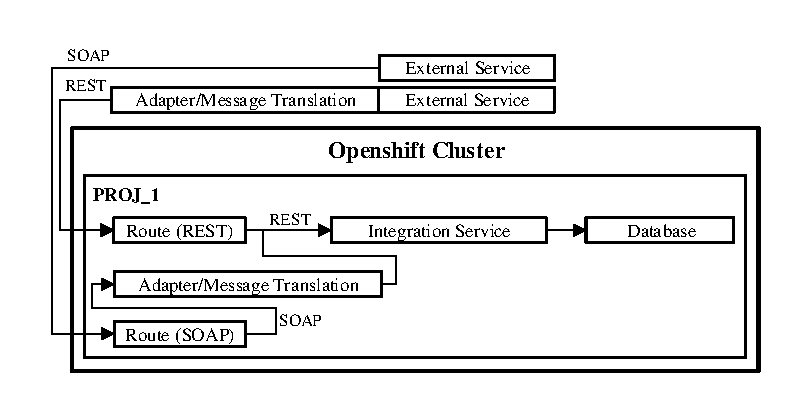
\includegraphics[scale=1]{images/esbd-service-adapter.pdf}
	\caption{External services integrated via an adapter}
	\label{fig:esbd-service-adapter}
\end{figure}

The Adapter and Message Translator have to be implemented as a standalone application (microservice), which for instance can be realized in Java with the Camel framework, which provides an API for implementing EI Patterns, and is capable of running as a standalone application. The adapter and message translator application can be hosted as a separate Openshift Service, or can be added to the service Pod as a so called side-by container, which proxies the requests to the actual container.  \\

\section{Further Work}
\label{sec:esbd-furhter-work}
During writing this thesis and the implementation of the prototype, Red Hat has released its new version of the JBoss Fuse platform, which now is based on Openshift, and is called Red Hat Fuse 7. Red Hat Fuse 7 enhances Openshift with features for implementing an ESB, whereby the main goal is to provide non-technical personal the possibility to create integrations. Red Hat Fuse 7 provides IPaaS features, by providing a low/no code UI, which allows to create integrations without the need to write a single line of code. \\

The next step is to implement an ESB with Red Hat Fuse 7, to see the differences between the manual approach, represented by the prototype, and the approach using IPaaS provided features. Red Hat Fuse 7 should make it easier for enterprises to create integrations to external services, as well as the management of these integrations.   

%%%----------------------------------------------------------
\appendix                                         % appendix 
%%%----------------------------------------------------------

%\chapter{Technical Details}
\label{app:TechnicalDetails}



	% technical supplements
%\chapter{CD-ROM/DVD Contents}
\label{app:cdrom}


	% contents of the CD-ROM/DVD
%\chapter{Questionnaire}
\label{app:Questionnaire}





	% chronological list of changes
%\chapter{\latex Source Code}
\label{app:SourceCode}

	% source text of this document

%%%----------------------------------------------------------
\MakeBibliography                     				% references
%%%----------------------------------------------------------
%%% special page for checking print size --------------------
%\chapter*{Check Final Print Size}

\begin{center}
{\Large --- Check final print size! ---}

\bigskip

\calibrationbox{100}{50} % width/height of box in mm

\bigskip

{\Large --- Remove this page after printing! ---}

\end{center}



%%%----------------------------------------------------------
\end{document}
%%%----------------------------------------------------------